\section{Architectural Design}
\subsection{Overview}

\begin{figure}[H]
    \centering
    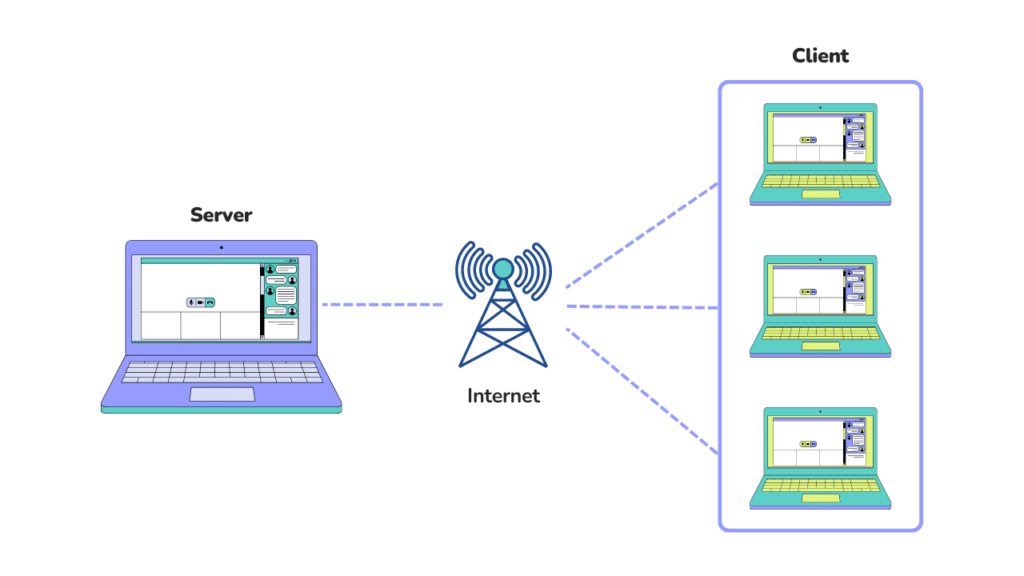
\includegraphics[width=0.75\textwidth]{Design/client-server-architecture-1024x576.png}
    \caption{Client-Server architecture}
    \label{fig:enter-label}
\end{figure}
Il sistema è un'applicazione distribuita che segue il noto paradigma client-server. Adotta la tecnica del thin client per facilitare il supporto di diverse piattaforme client. Questo approccio offre vantaggi significativi: primo, riduce i requisiti di hardware e software sui dispositivi client, poiché l'elaborazione principale è gestita dal server. Questo significa che anche i client con capacità di elaborazione limitata possono accedere efficacemente al sistema. Secondo, semplifica notevolmente la manutenzione e l'aggiornamento del software, in quanto le modifiche sono centralizzate sul server e non devono essere implementate su ogni dispositivo client individualmente. Infine, migliora la sicurezza, poiché i dati sensibili possono essere memorizzati e gestiti in modo più sicuro sul server, riducendo il rischio di perdite di dati o violazioni della sicurezza sui dispositivi client. Il nostro sistema utilizza come client le applicazioni web.

\noindent \textbf{Tier architecture} \\
\noindent The architecture of our system is organised into four tiers:
\begin{enumerate}
    \item Thin Client: Il Thin Client è il punto di contatto con l'utente, come ad esempio un  un browser web.
    \item Web Server: Il Web Server funge da intermediario tra il client e l'Application Server. È responsabile della ricezione delle richieste HTTP/HTTPS dal Thin Client  e dell'inoltro delle richieste elaborate all'Application Server. 
    \item Application Server: L'application Server è il cuore del sistema, dove la logica di business e le funzionalità dell'applicazione sono elaborate. Questo tier elabora le richieste provenienti dal Web Server, eseguendo operazioni complesse, gestendo la logica di business, le transazioni e l'interazione con il Database Server. L'Application Server può ospitare una varietà di servizi web, microservizi, e API che espongono la funzionalità dell'applicazione al Web Server e, di conseguenza, al Thin Client.
    \item Database Server: Il Database Server gestisce la persistenza, il recupero e la gestione dei dati.
\end{enumerate}


\begin{figure}[H]
    \centering
    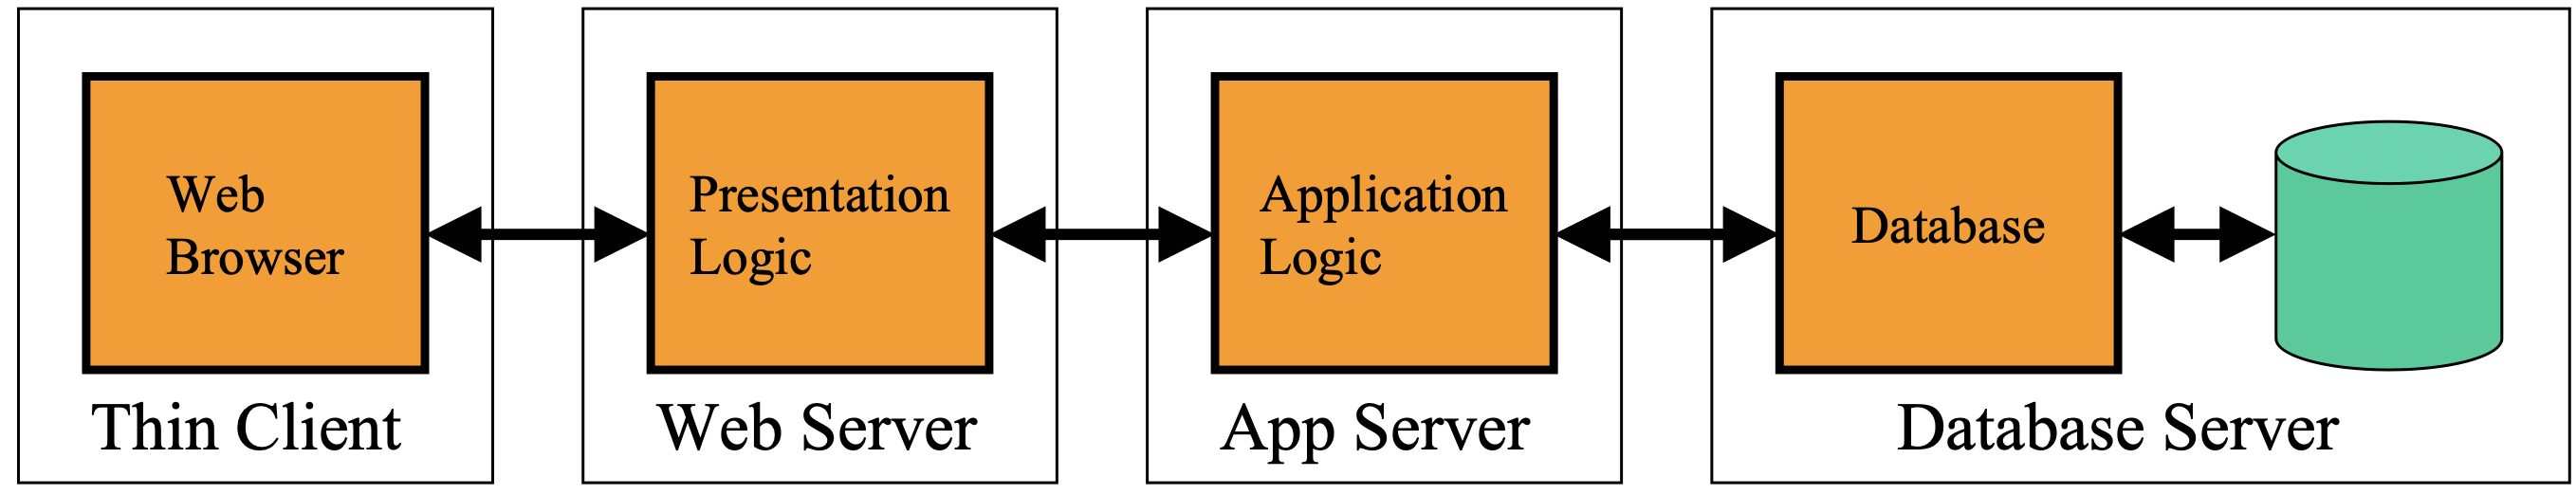
\includegraphics[width=0.75\textwidth]{Design/Screenshot 2023-12-23 at 10.54.18.png}
    \caption{4 Tier architecture}
    \label{fig:enter-label}
\end{figure}


\newpage
\noindent \textbf{Layers architecture}\\
An application consists of layers  representing the different levels and types of abstraction of the software. The layers help to slice the application into more manageable units and support multiple implementations.
 The logical software architecture of our system consists of three layers:
\begin{enumerate}
    \item Presentation layer: manages the presentation logic and the user interaction.
    \item Application layer: manages the business logic and functions that the system must provide.
    \item Data layer: manages the storage and retrieval of data.
\end{enumerate}


\begin{figure}[H]
    \centering
    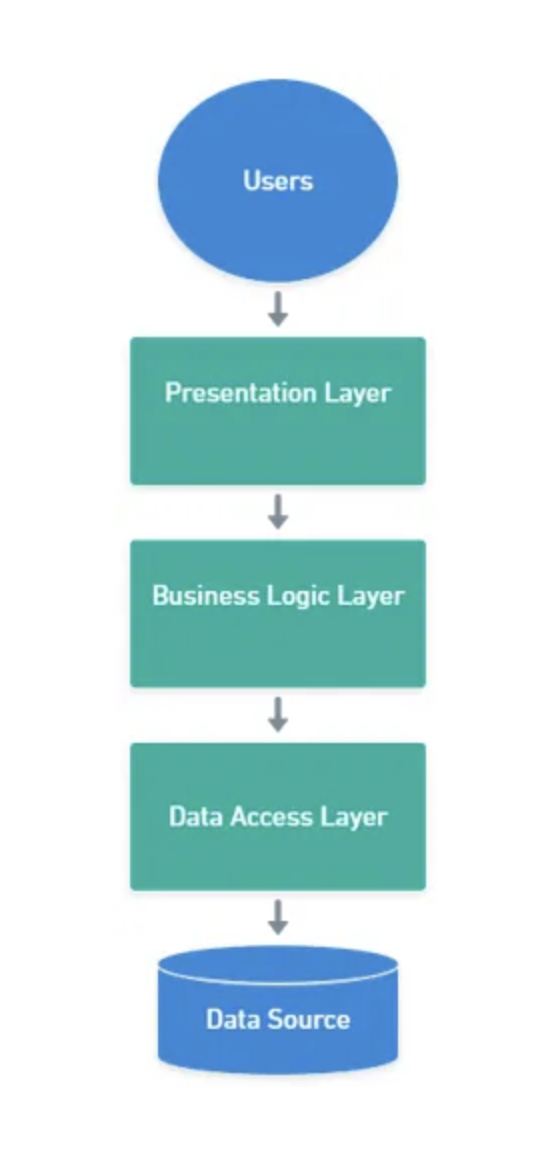
\includegraphics[width=0.3\textwidth]{Design/threeLayer.png}
    \caption{3 Layers architecture}
    \label{fig:enter-label}
\end{figure}


The first two tiers are used for the presentation layer, while the 3rd tier is for the application layer and the 4th tier is for the data layer.

The system architecture requires the client to interact with web servers. These servers act as an intermediate layer, facilitating communication between the client and the application layer via well-defined APIs. The application layer, in turn, communicates with the data layer via Database Management System (DBMS) APIs.

To ensure ease of portability and scalability, the APIs on the application server are designed to be RESTful. Such APIs are simple, standardised and stateless. This design choice increases flexibility and allows for easier integration of client code. When it comes to interacting with the data layer, we use Object-Relational Mapping (ORM) techniques. This approach exploits the principles of object-oriented programming, allowing seamless access to a relational database.

As far as security is concerned, each physical layer of the system is isolated by a dedicated firewall. In addition, all communication between these layers is encrypted, adhering to the HTTPS standard for secure data transmission.



\begin{figure}[H]
    \centering
    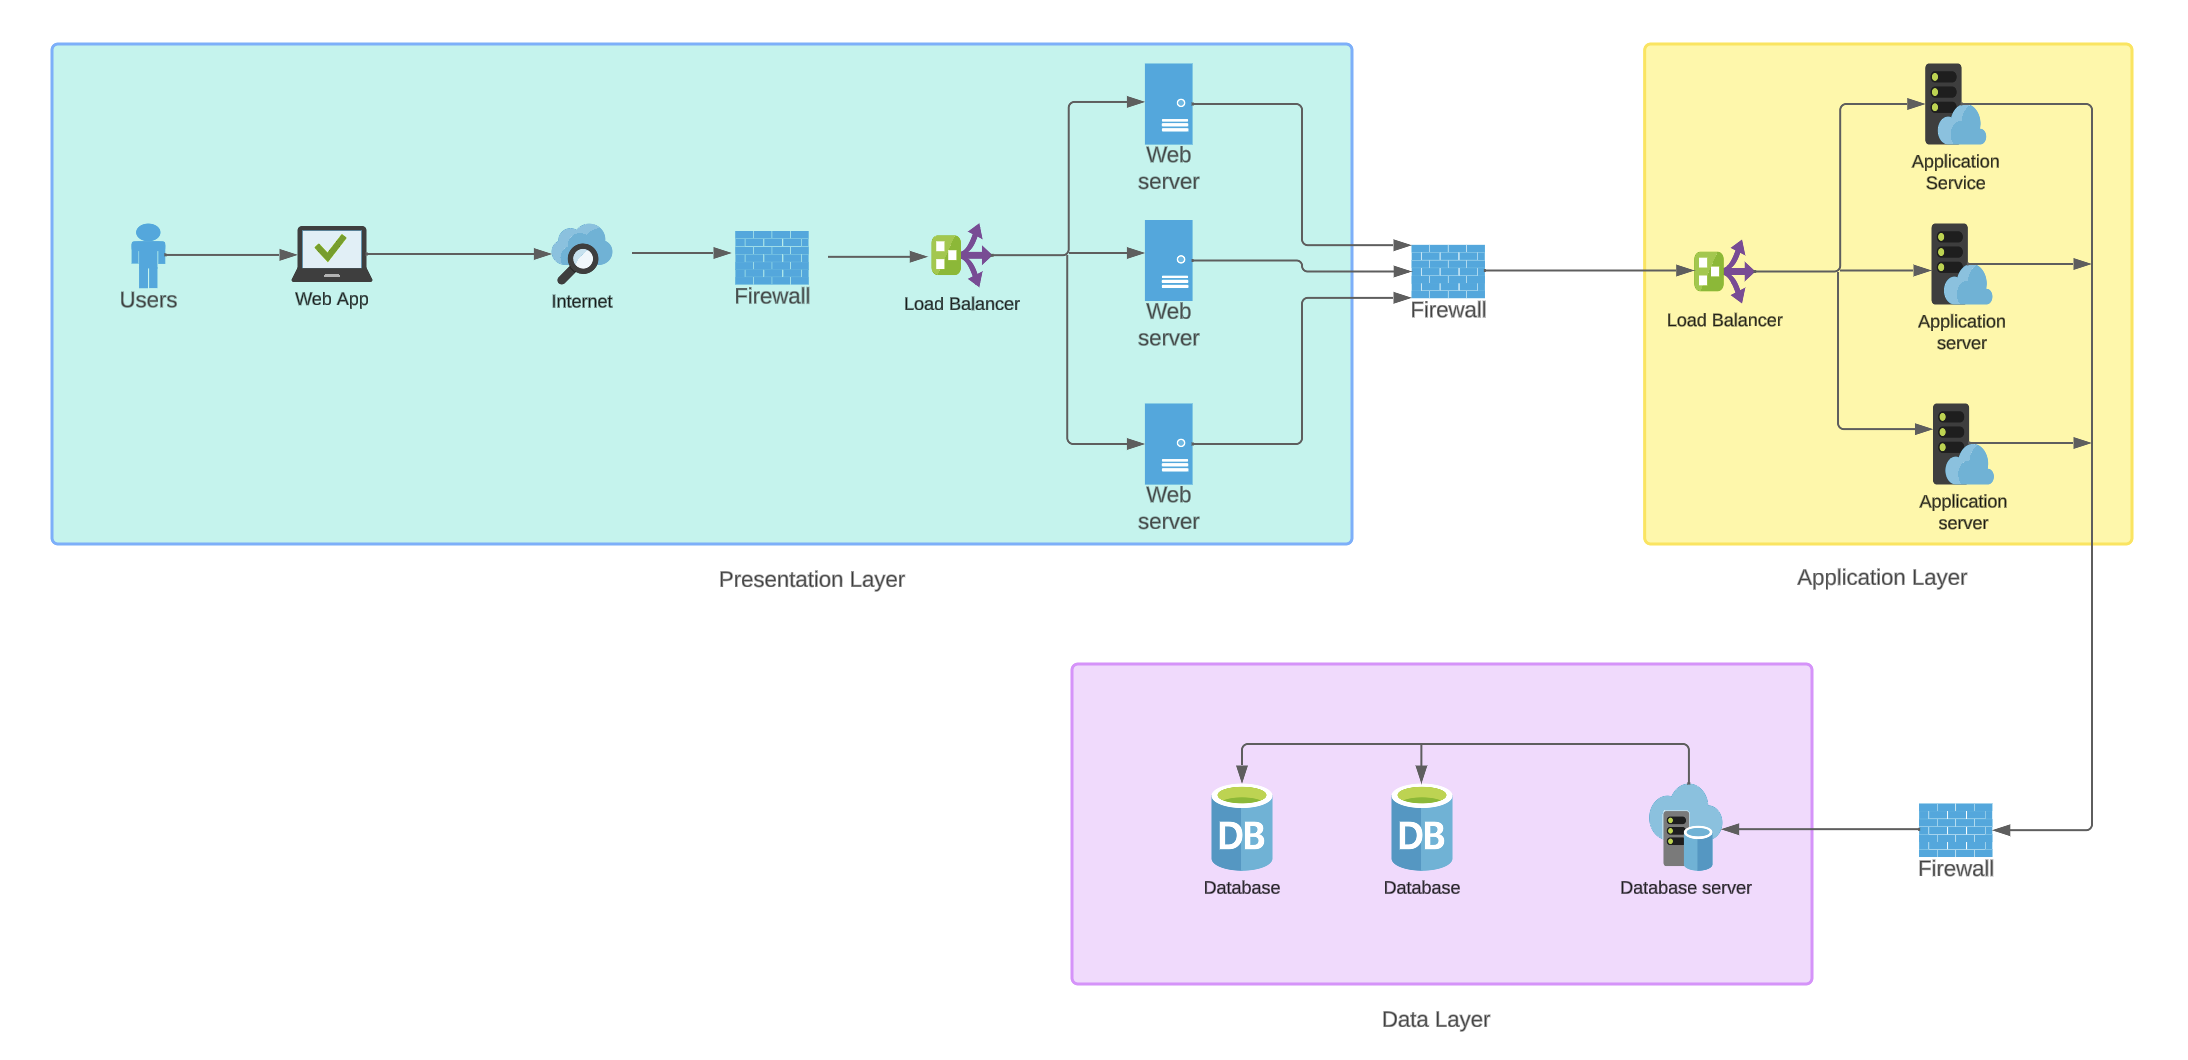
\includegraphics[width=0.9\textwidth]{Design/ArchitectureFinal.png}
    \caption{Architecture}
    \label{fig:enter-label}
\end{figure}


\noindent \textbf{Load Balancing}\\
\noindent Nella architettura presentata ci sono due load balancer che svolgono ruoli cruciali nel gestire il traffico in ingresso verso i server web e applicativi.
\begin{enumerate}
    \item Primo Load Balancer: Situato dopo il firewall e prima dei server web, questo load balancer ha il compito di distribuire le richieste dei client in arrivo  ai server web. Quando una richiesta passa attraverso il firewall, viene intercettata dal load balancer, che poi determina quale server web è il più idoneo per gestire quella richiesta. Il criterio di scelta è basato sul carico corrente di ciascun server e  sulla capacità di minimizzare il tempo di risposta. In questo modo, il bilanciamento del carico aiuta a prevenire il sovraccarico di un singolo server web, garantendo una distribuzione equa delle richieste e ottimizzando l'utilizzo delle risorse.
    \item Secondo Load Balancer: Situato tra i server web e i server applicativi, il secondo load balancer agisce in modo simile al primo, ma a un livello diverso dell'architettura. Dopo che il server web ha elaborato la richiesta iniziale  la inoltra al secondo load balancer. Quest'ultimo poi distribuisce la richiesta a uno dei server applicativi disponibili, ancora una volta basandosi sul carico di lavoro e sulla capacità di fornire una risposta rapida. In questo modo, anche il livello applicativo è protetto dal rischio di sovraccarico e può scalare efficacemente in risposta a variazioni del traffico.
\end{enumerate}
\leavevmode 
\newline
In the following sections, each component of the system will be elaborated in more detail, providing a complete understanding of the entire architecture.

\subsection{Component View}
\begin{figure}[H]
    \centering
    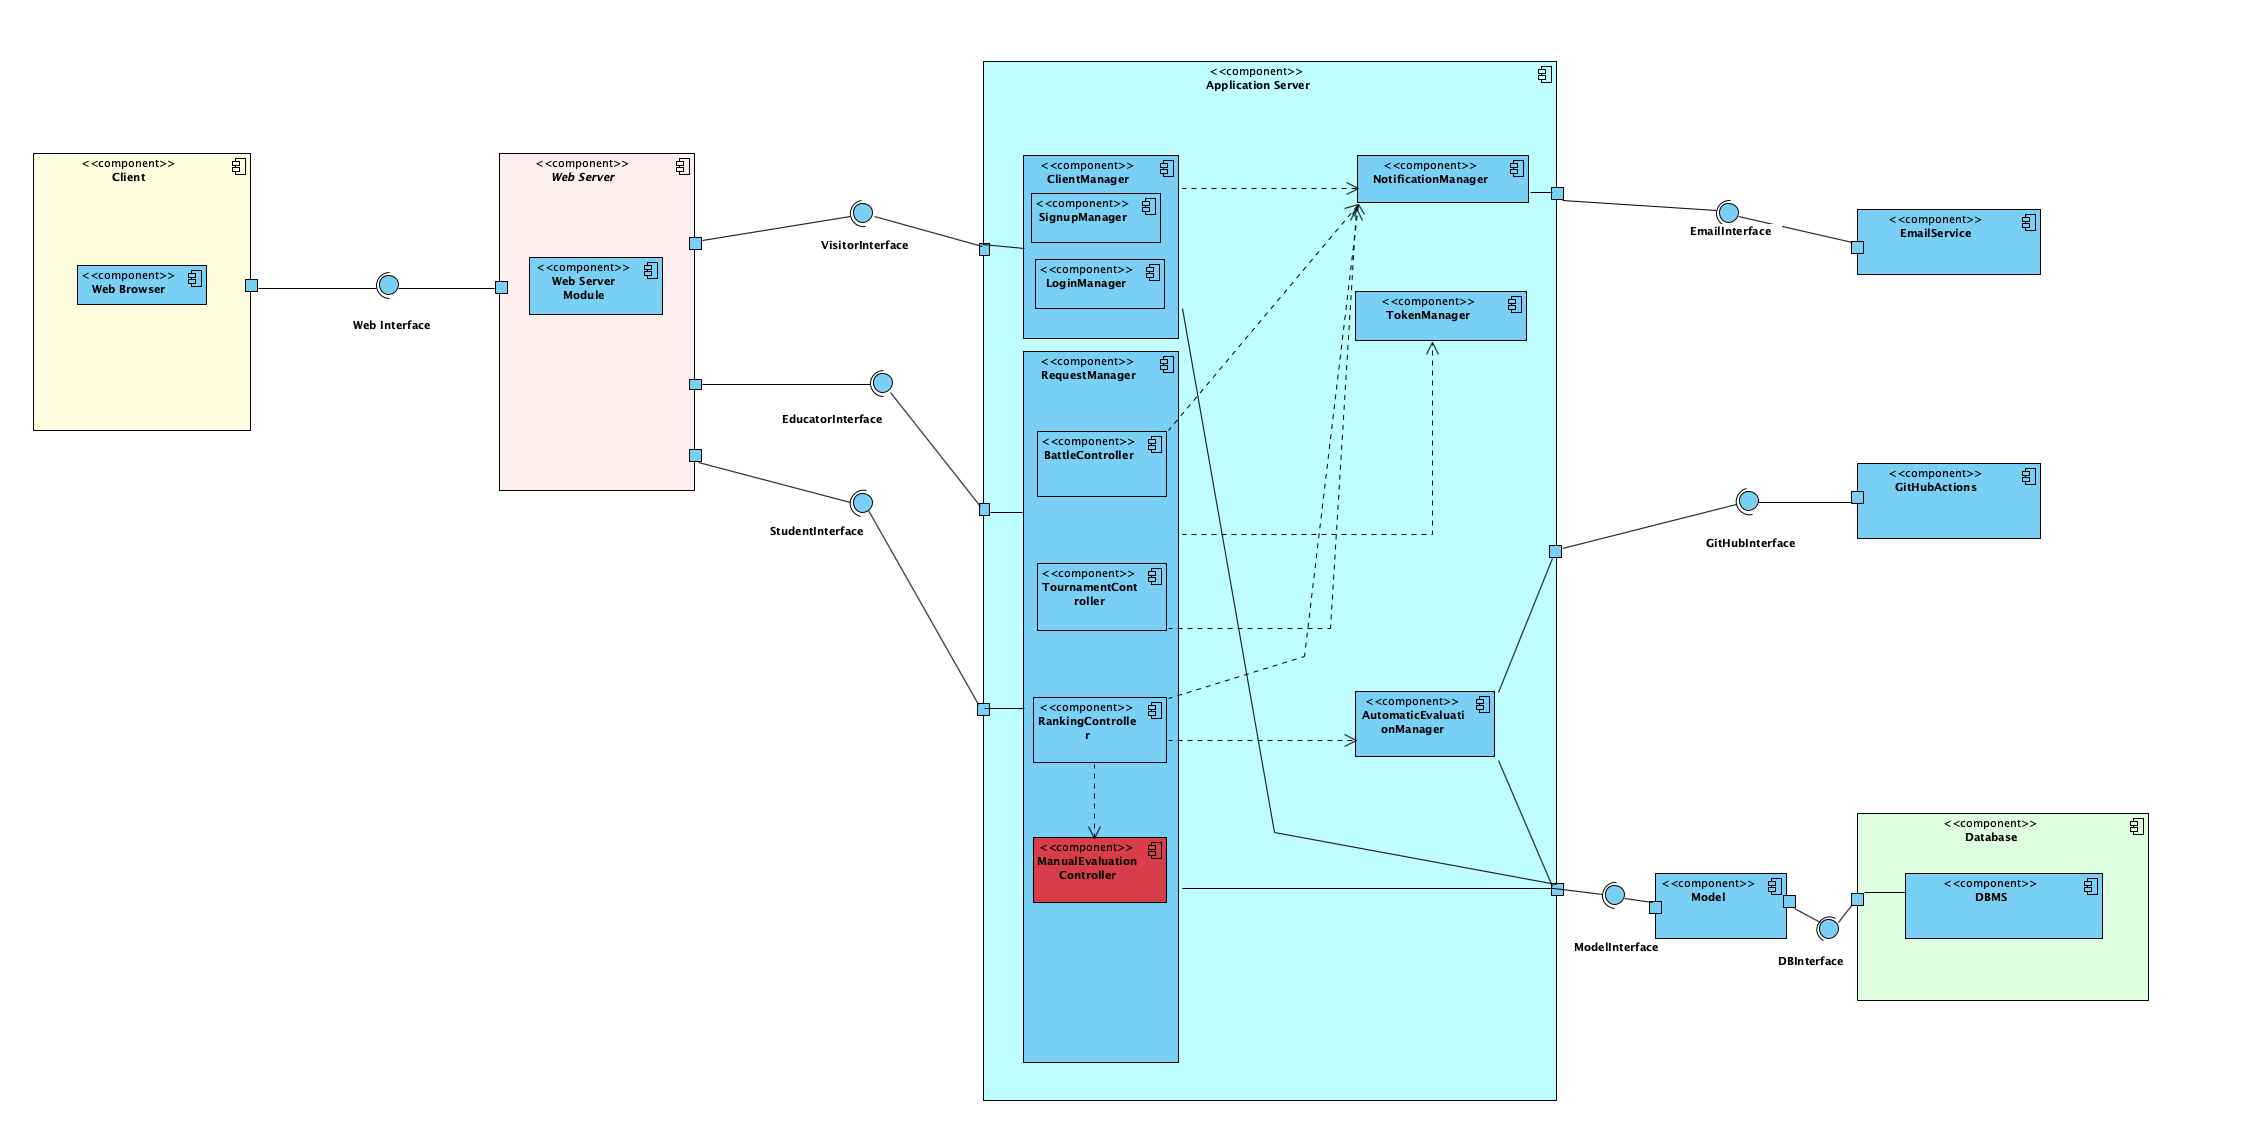
\includegraphics[width=1.1\textwidth]{Design/ComponentDiagram.png}
    \caption{3 Layers architecture}
    \label{fig:enter-label}
\end{figure}
Breve descrizione dei componenti più importanti:
\begin{itemize}
    \item Web Server: it handles managing HTTP requests from the client and forwarding them to the application server.
    \item Client Manager: it manages all requests from users who are not yet authenticated, giving them the opportunity to register (Signup Manager) or log in (Login Manager). To handle all requests, it utilizes the login interface and registration interface and issues authentication tokens that are useful for other services. The token is also used to identify whether the user is a student or educator.
\item Request Manager: It verifies that each request comes from a user who has logged in using the token manager and then redirects each request to the appropriate controller.

\item BattleController: It is responsible for managing all functionalities related to battles, such as creating new battles, creating a team, participating in new battles, etc.

\item TournamentController: It is responsible for managing all functionalities related to tournaments, such as creating new tournaments, participating in new tournaments, etc.

\item RankingController: It is responsible for managing ranking functionalities, such as displaying real-time scores for each team in each battle, displaying scores for each student in each tournament, etc.

\item ManualEvaluationController: It allows only educator-type users to assign a score to each student's task for a specific battle where manual evaluation is enabled.

\item AutomaticEvaluationManager: It is responsible for the automatic calculation of the project score for each team upon submission to GitHub by the teams participating in a specific battle. This controller is triggered by GitHub Actions.

\item Token Manager: It manages the creation, validation, renewal, and revocation of authentication tokens.

\item NotificationManager: It handles the management of notifications whenever requested. Notifications are sent via email through the Email Service.

\item Model: serves as the repository for data that constitute the enduring state of the system, which, in our scenario, is preserved within a database. When the application initiates, this component ensures the data are loaded for use. It encompasses a suite of methods essential for accessing this data and encapsulates the logic necessary for their manipulation. Essentially, when any system component requires database information for computational purposes, it entrusts the Model component with the retrieval task. The Model not only fetches the requisite data but also organizes them into specialized data structures, thus priming them for imminent computational tasks. It is the sole component that interfaces with the database management system (DBMS), acting as the exclusive conduit for data interaction.
    
\end{itemize}

\subsection {Deployment View}
\begin{figure}[H]
    \centering
    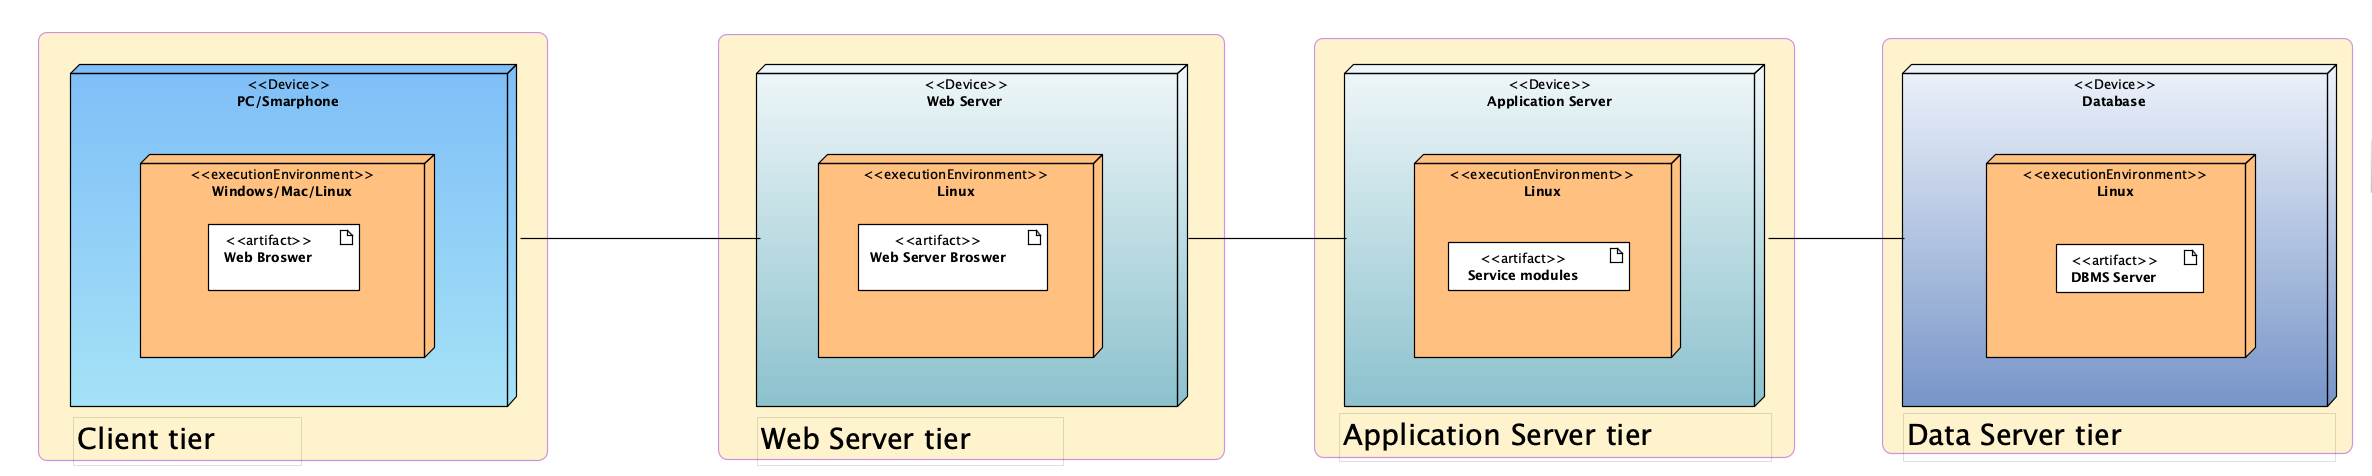
\includegraphics[width=1.1\textwidth]{Design/DeploymentView.png}
    \caption{Architecture}
    \label{fig:enter-label}
\end{figure}
The diagram presented shows the organisation of the system, highlighting the components required for its operation. Each device illustrated runs a specific operating system that supports the execution of the software components. To expand the system, additional copies of these devices can be added.
The tiers are four:
\begin{itemize}
    \item \textbf{Client tier}:  Questo strato include dispositivi come PC e smartphone che utilizzano sistemi operativi come Windows, Mac o Linux. Il componente software principale in questo livello è il browser web, che permette agli utenti di interagire con il sistema.
    \item \textbf{Web server tier}:Questo livello è costituito da server web che eseguono un sistema operativo Linux. Il componente software rappresentato è Apache che si occupa di elaborare le richieste dei client e servire pagine web.

    \item \textbf{Application server tier}:  Questo strato include server di applicazioni, anch'essi su Linux, che eseguono moduli di servizio. Questi moduli gestiscono la logica di business dell'applicazione e di solito comunicano tra il web server e il database server.
    \item \textbf{Data server tier} :  L'ultimo livello è composto da un database che gira su Linux, con un DBMS (Database Management System) Server come componente software. Questo gestisce lo storage e il recupero dei dati.
\end{itemize}
\subsection{Runtime views}
This chapter details the dynamic perspectives linked to the use cases outlined in the RASD for CKB. It illustrates how different components interact to facilitate the functions provided by CKB, offering a comprehensive look at its operational architecture.
\subsubsection{Educator Registration}
\begin{figure}[H]
    \centering
    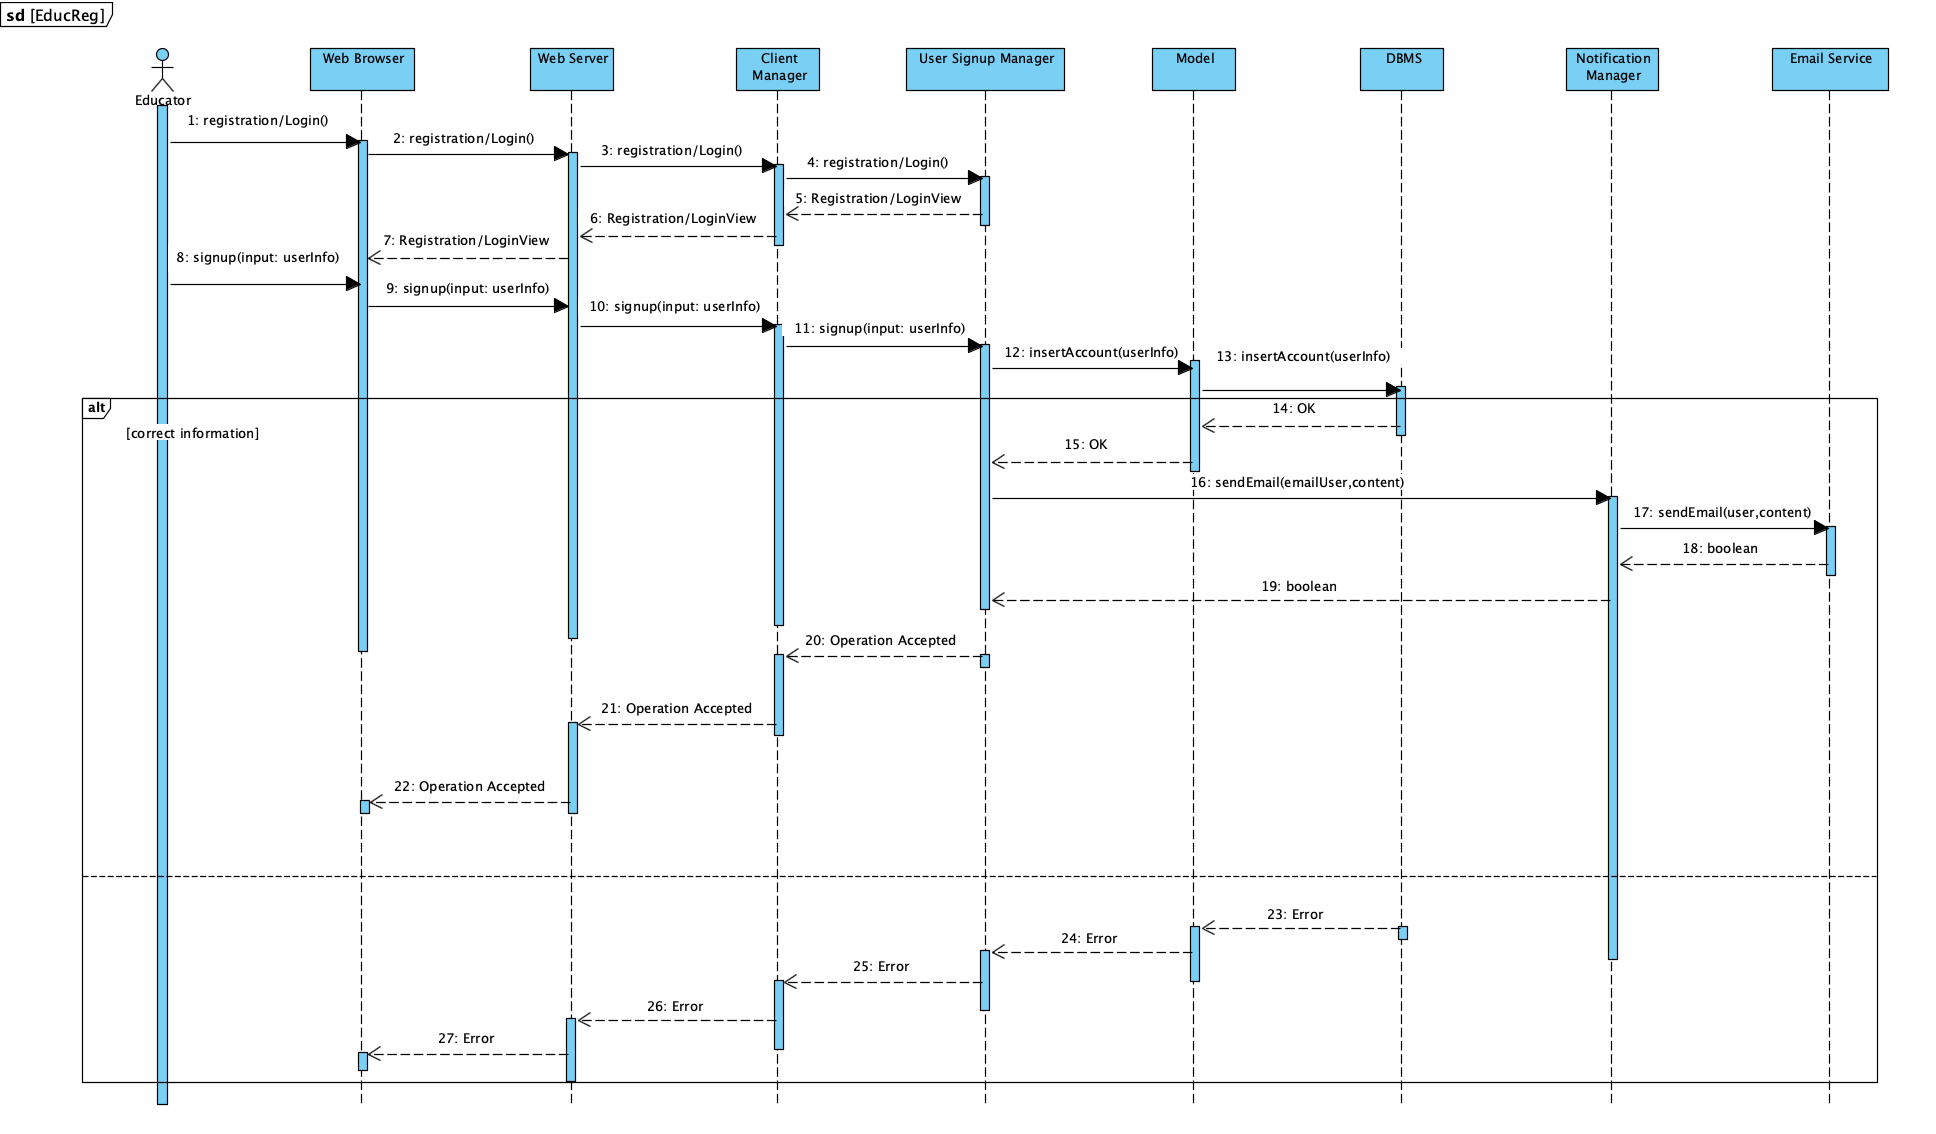
\includegraphics[width=1\textwidth]{SequenceDiagram/EducatorReg.png}
    \label{fig:enter-label}
\end{figure}

The sequence diagram depicted shows the registration flow of an educator. The educator starts the process from the homepage by clicking on the 'Registration/Login' section. The system offers the options of registration or login. Upon choosing registration, the educator is presented with a form to complete and a box to tick if he/she is an educator. After entering the data, the educator confirms registration. The system verifies the data and invites the educator to check his/her mailbox to confirm the registration via a link sent by the platform. If the data is incorrect, the DBMS sends an error message that propagates to the Web Browser. On the backend, components such as the Web Server, the Client Manager, and others manage the registration process, from creating the account to entering the data in the archive, to sending an email for verification. Once the educator confirms registration via email, his or her data is entered into the database, successfully completing the registration process.


\subsubsection{Student Registration}
\begin{figure}[H]
    \centering
    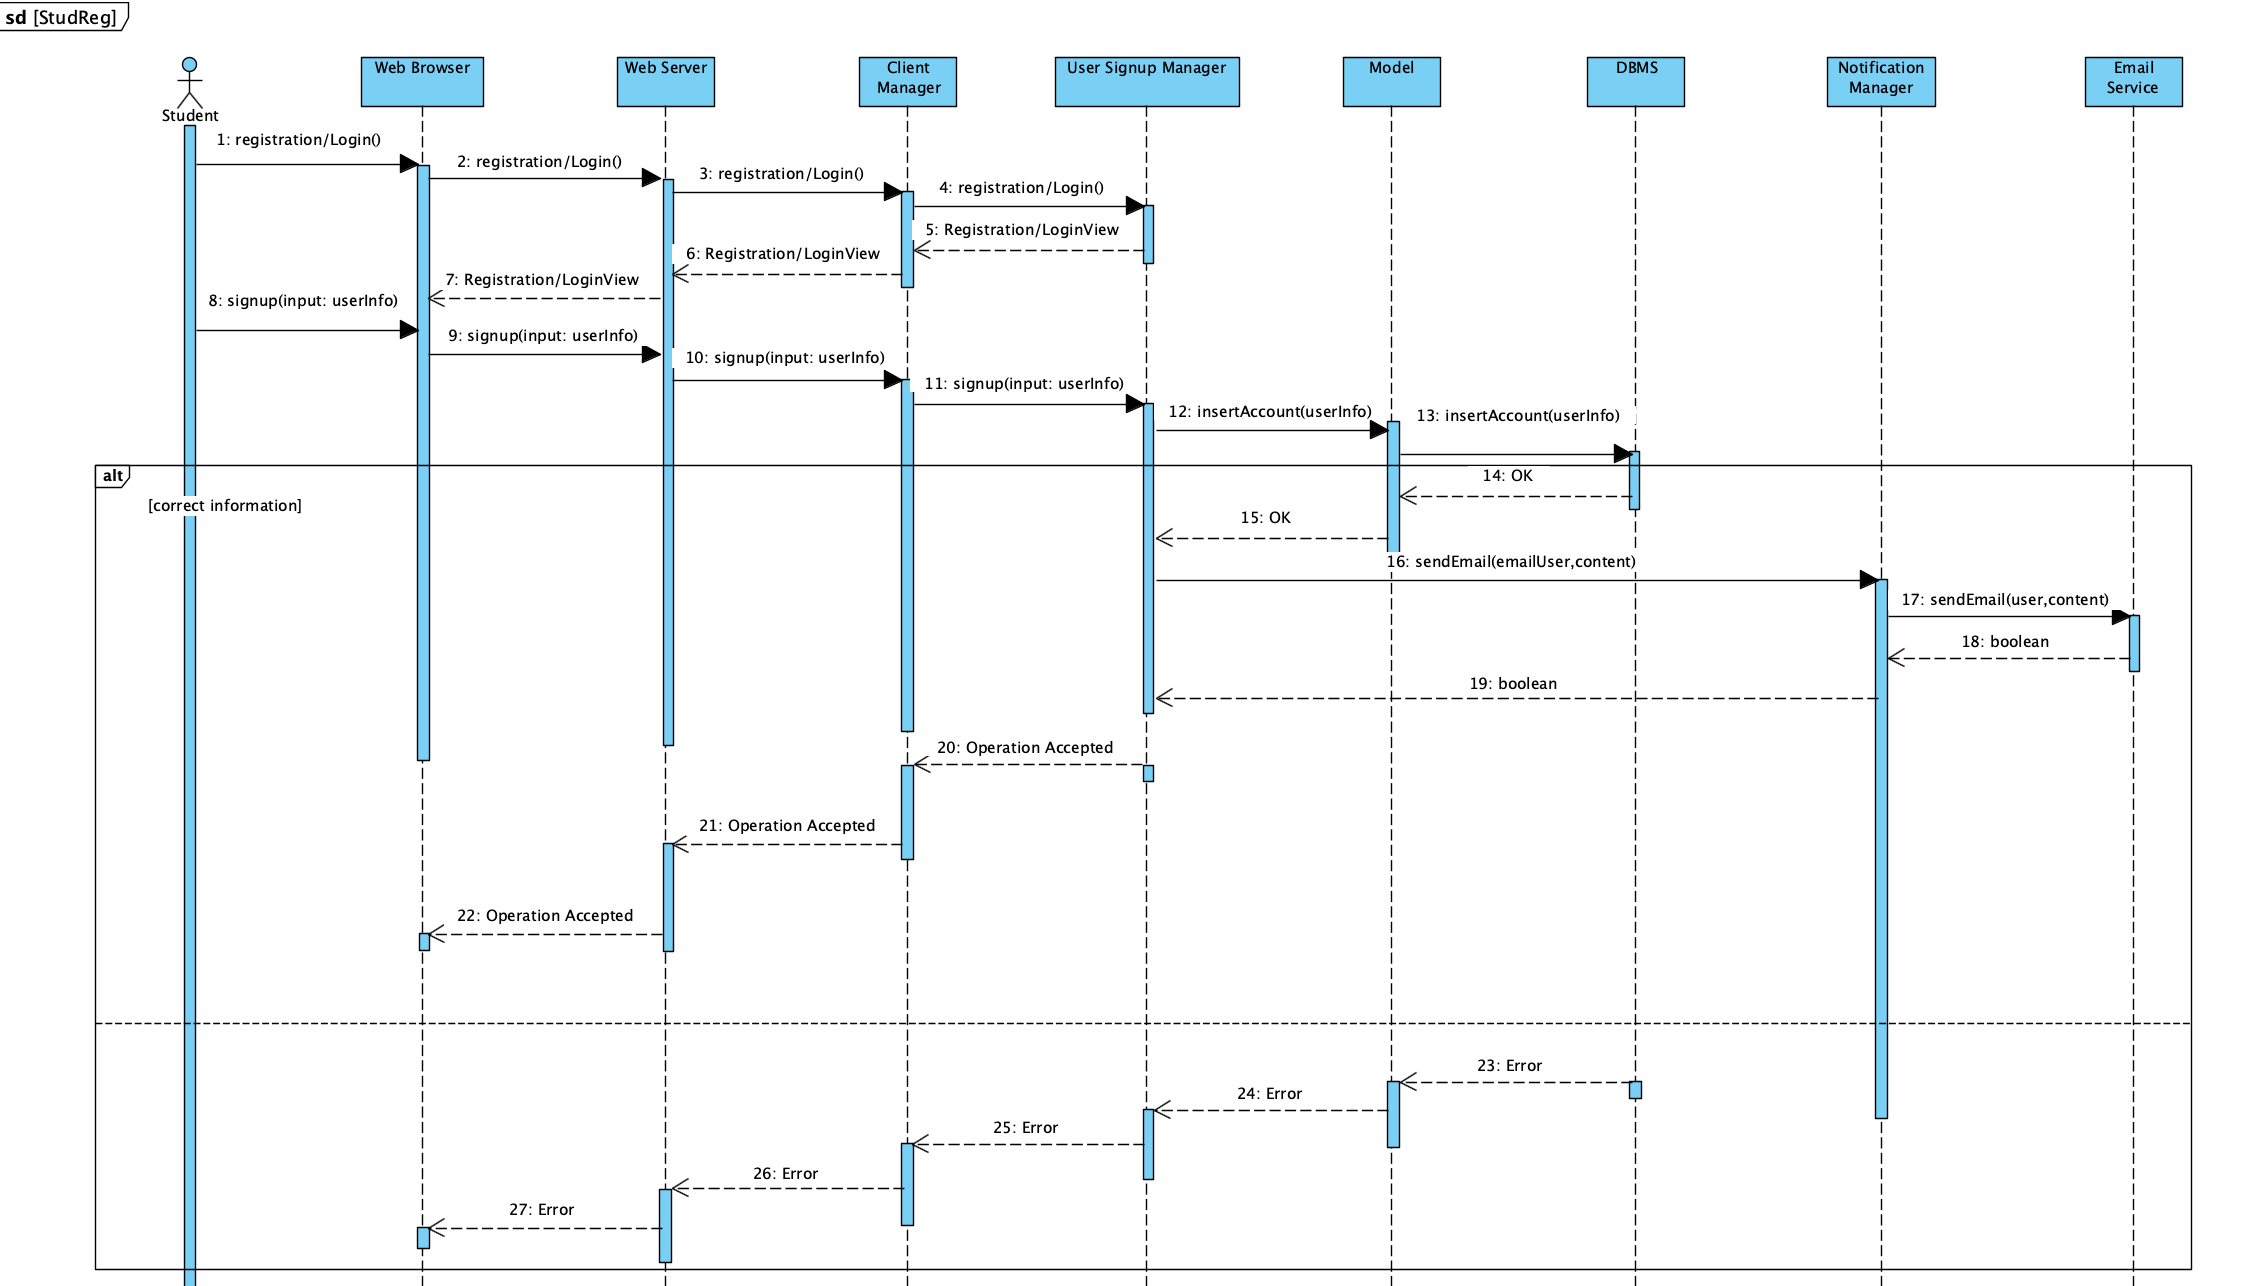
\includegraphics[width=1\textwidth]{SequenceDiagram/StudReg.png}
    \label{fig:enter-label}
\end{figure}
In the sequence diagram displayed, a student initiates registration via the homepage, completes a form with his or her personal data and confirms registration. The Web Browser interacts with the Web Server, which in turn involves the Client Manager and the User Signup Manager to manage the sequence of events.
These components co-ordinate the registration operation, with the User Signup Manager sending the data to the Model layer, which forwards it to the Database Management System (DBMS) for actual entry of the information into persistent storage. The process continues with the generation of a confirmation email, which relies on the Notification Manager to send the message to the user. The flow ends when the student, by verifying and accepting the registration via the link received by email, activates the final entry of his or her data into the database. If, on the other hand, the data entered are found to be inadequate, an error message is sent.
\subsubsection{User Login}
\begin{figure}[H]
    \centering
    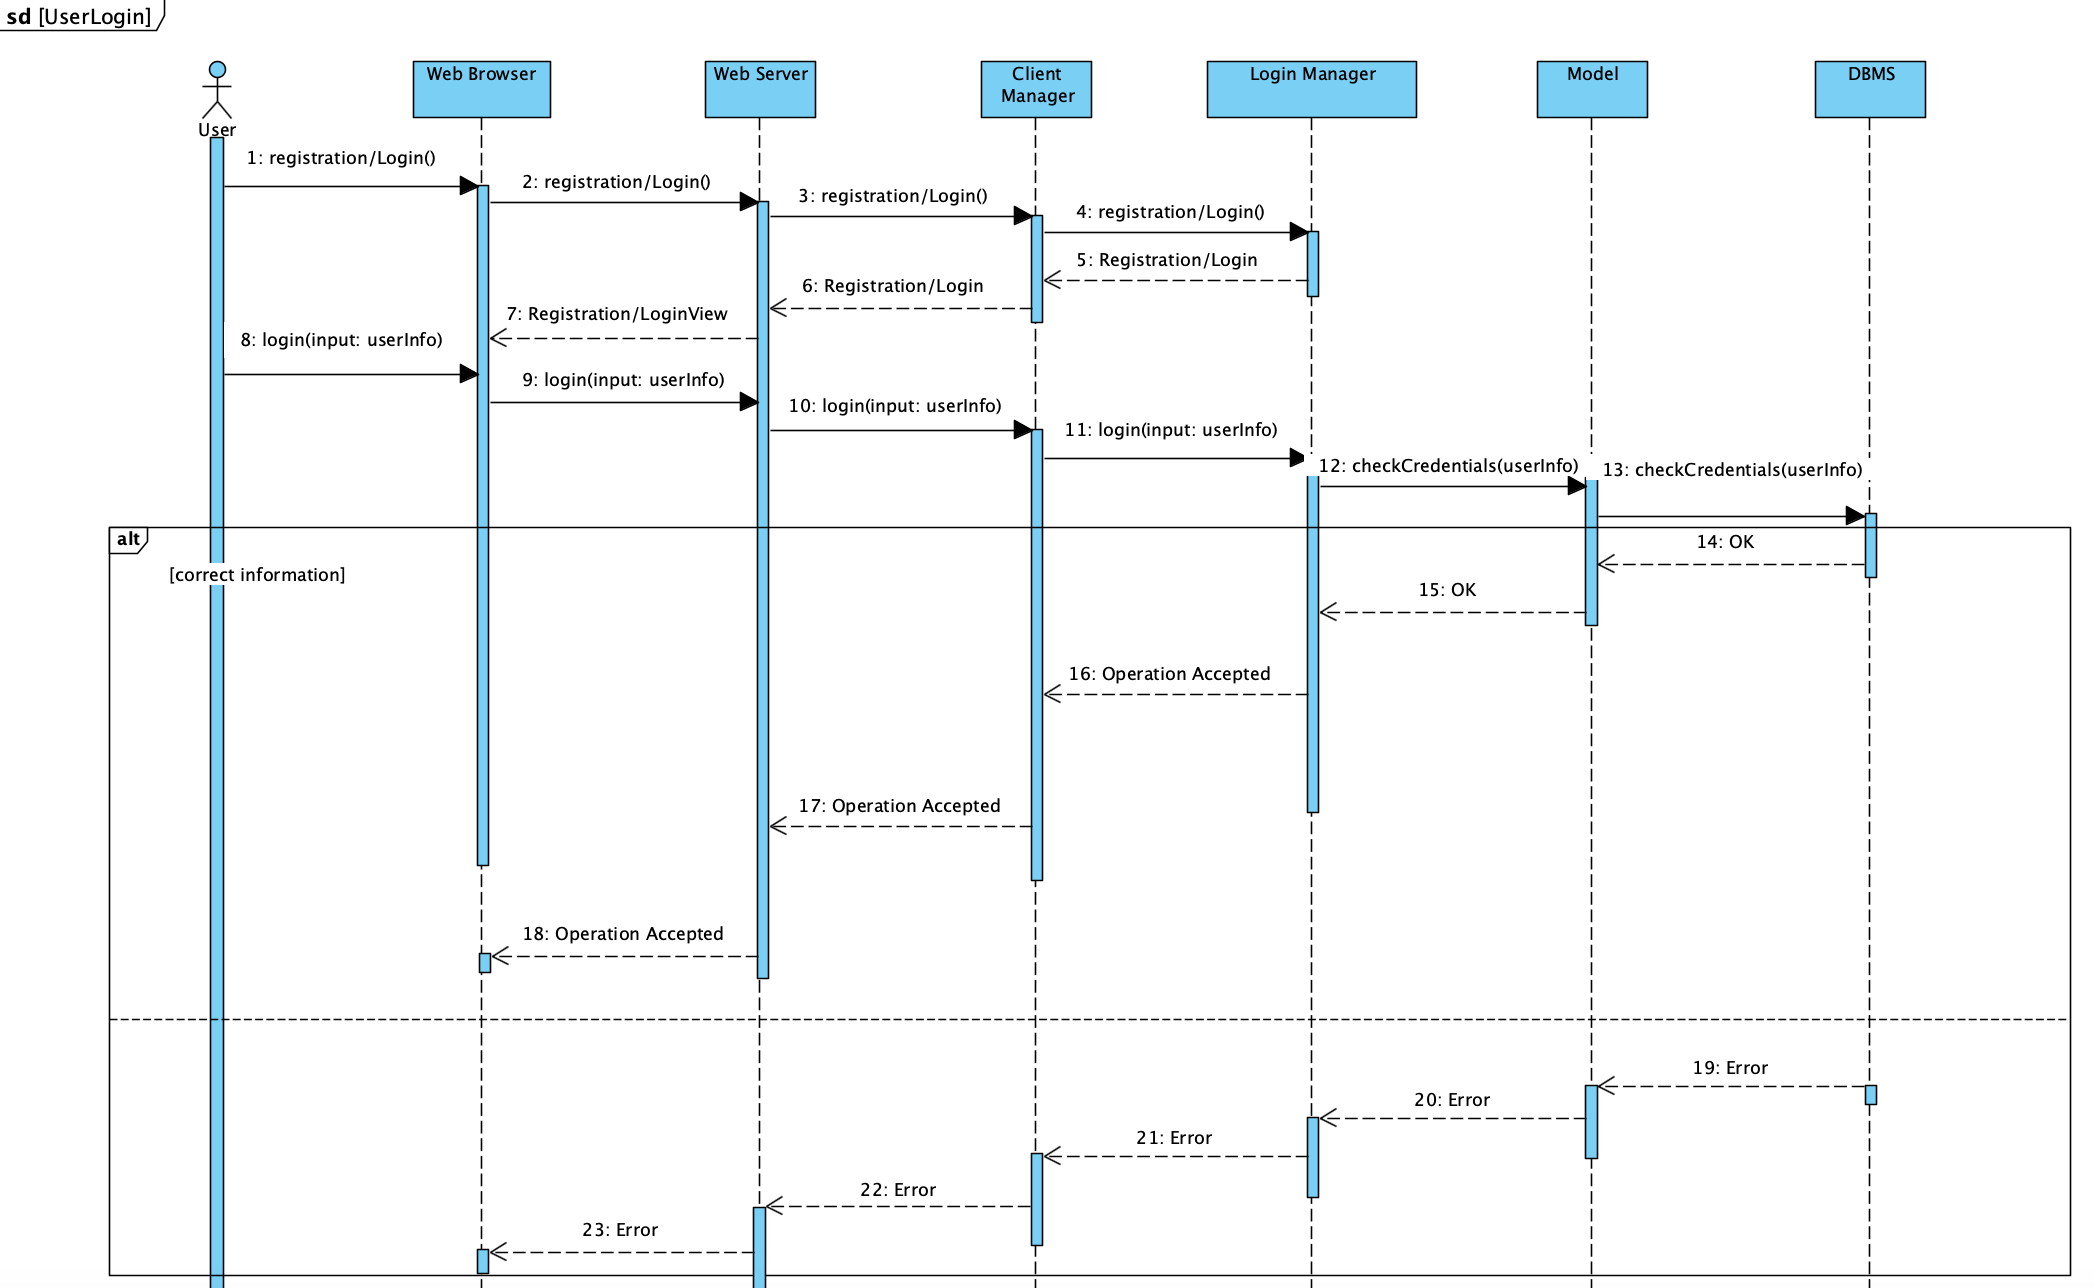
\includegraphics[width=1\textwidth]{SequenceDiagram/UserLogin.png}
    \label{fig:enter-label}
\end{figure}
The sequence diagram shown illustrates the login process of a user. The user starts by clicking on the "Registration/Login" section of the homepage, after which the system presents registration or login options. By choosing 'Login', the user is prompted to enter their email and password. Once the credentials have been entered and the "Confirm" button clicked, the system via the Web Server and Client Manager passes the information to the User Signup Manager. The latter component makes a call to the Model, which queries the DBMS to verify the user's credentials.
If the information is correct, the process ends with the transaction being accepted and the system grants the user access to their profile dashboard. Otherwise, an error is reported and the user cannot log in. 
\subsubsection{Tournament Creation}
\begin{figure}[H]
    \centering
    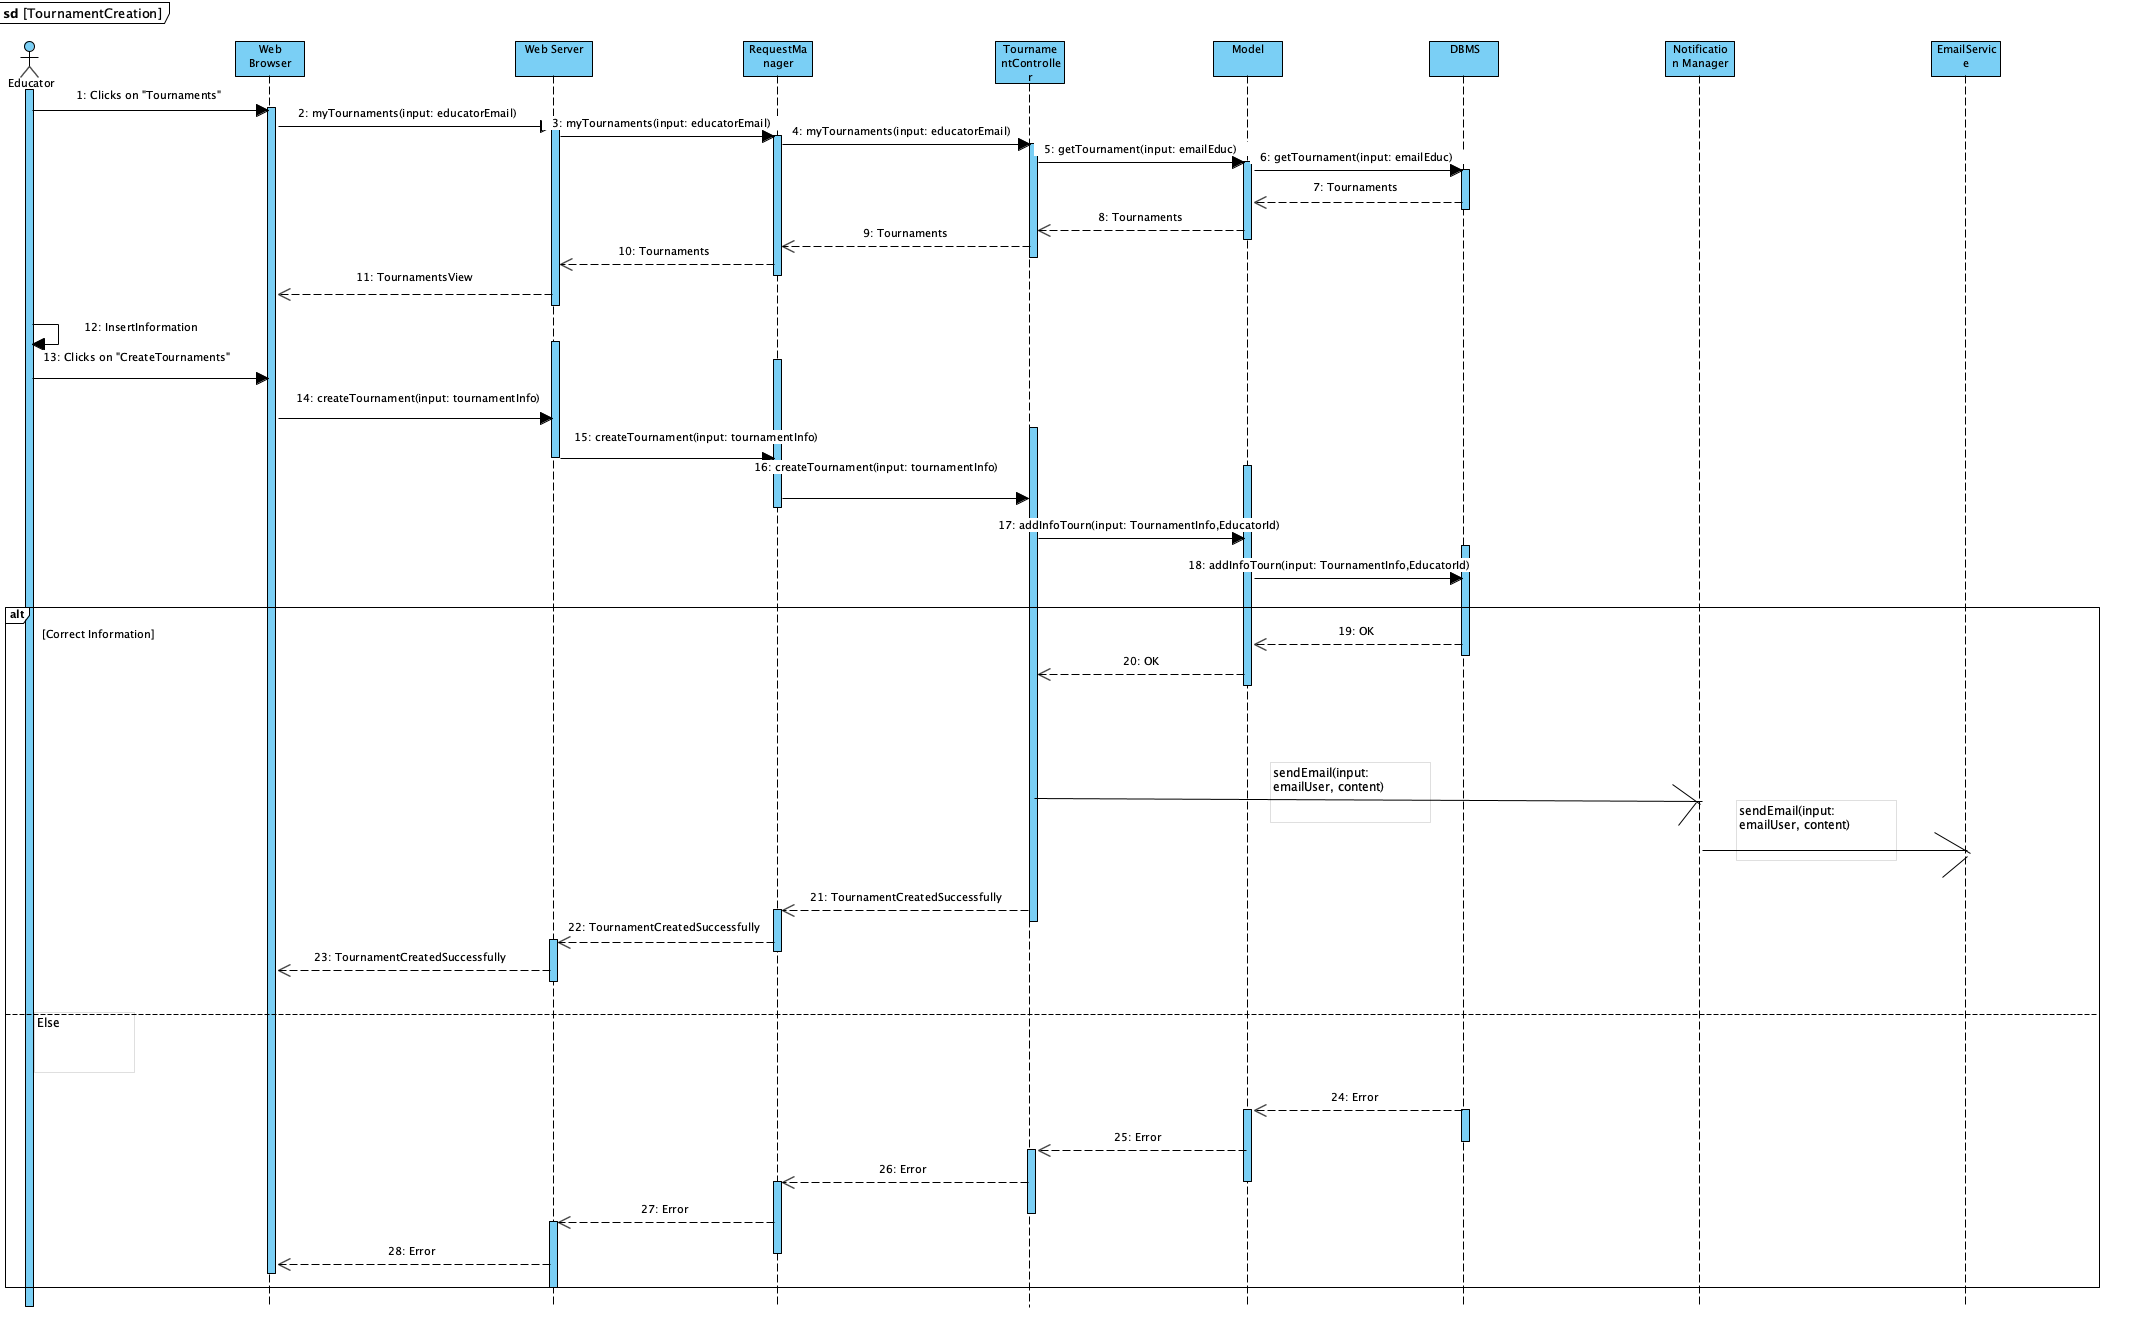
\includegraphics[width=1\textwidth]{SequenceDiagram/TournamentCreation.png}
    \label{fig:enter-label}
\end{figure}
The sequence diagram shows the process the educator follows to create a tournament on the platform. After selecting the option to create a tournament, the educator enters the required data via the Web Browser. This information is sent to the Web Server, which interfaces with the Request Manager. The Request Manager co-ordinates the data flow, sending the information to the Tournament Manager.

The Tournament Manager is responsible for the business logic related to the creation of tournaments. It communicates with the Model, which represents the logical structure of the data, and queries the DBMS to verify the existence and validity of the email addresses provided. Once the verification is complete, the Model updates the DBMS with the new tournament information.

Once the creation of the tournament is confirmed, the Notification Manager comes into play, invoking the Email service to notify students registered on the platform. The process concludes by saving the tournament information in the DBMS and notifying interested users, showing positive feedback through the educator user interface.
\subsubsection{Battle Creation}
\begin{figure}[H]
    \centering
    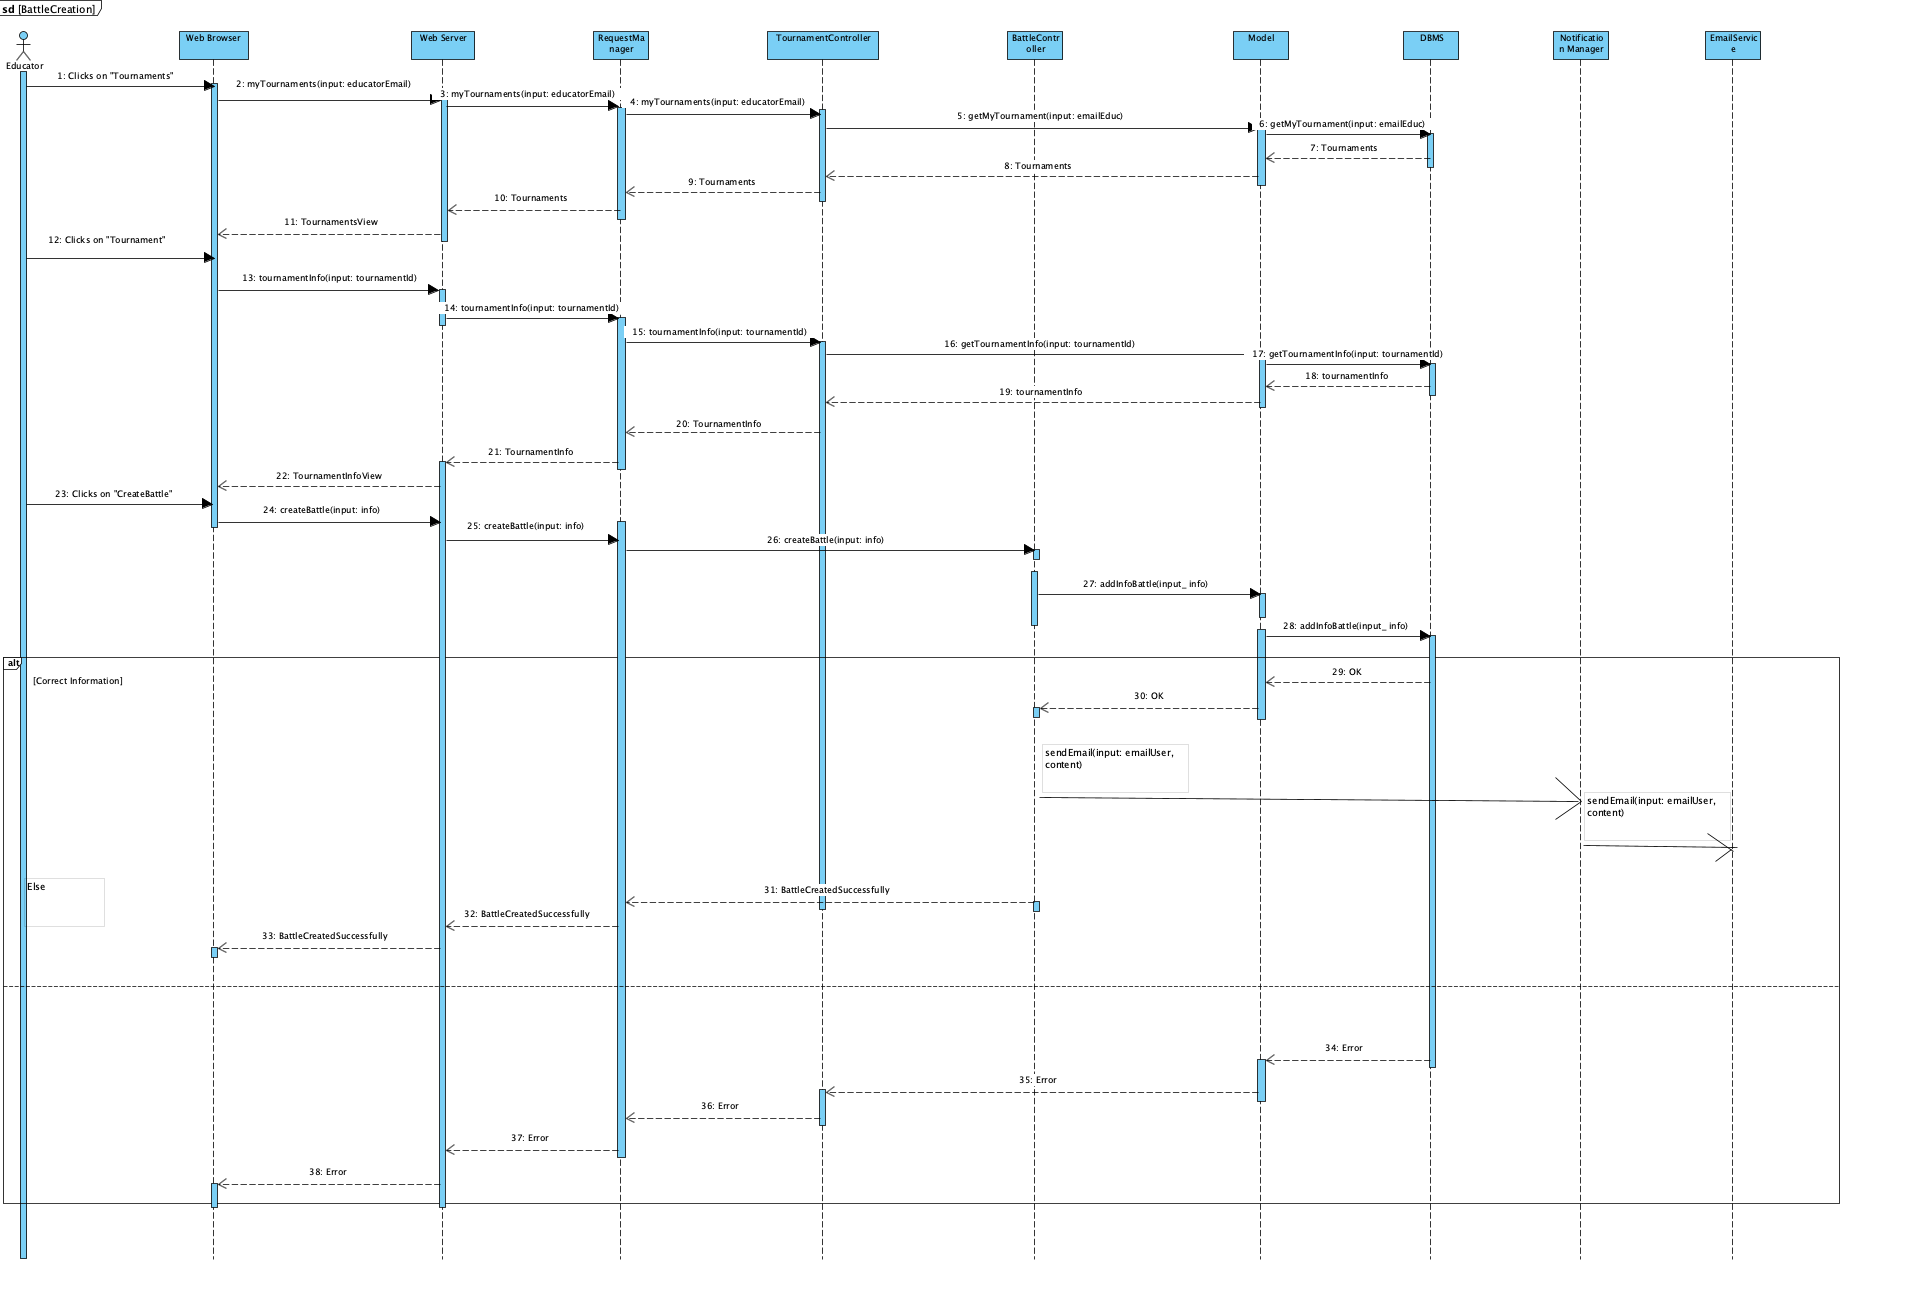
\includegraphics[width=1\textwidth]{SequenceDiagram/BattleCreation.png}
    \label{fig:enter-label}
\end{figure}
In the sequence diagram, the educator interacts with the system to create a battle within a tournament. This interaction begins in the Web Browser and is sent to the Web Server, which acts as a conduit for all subsequent requests and responses.
The flow continues with the Request Manager which processes the request to create the battle, routing it to the Tournament Controller. The latter has the task of managing the tournament-specific data and interfaces with the Model to manipulate the logical structure of the data.
The Model communicates with the DBMS to verify the uniqueness of the battle name and, if valid, to store the new information in the database. Once the DBMS confirms the addition of the data with an 'OK', the Notification Manager is activated.
The Notification Manager coordinates with the Email service to send notifications to students registered for the tournament, informing them of the newly created battle. 
\subsubsection{Student registers for the Tournament}
\begin{figure}[H]
    \centering
    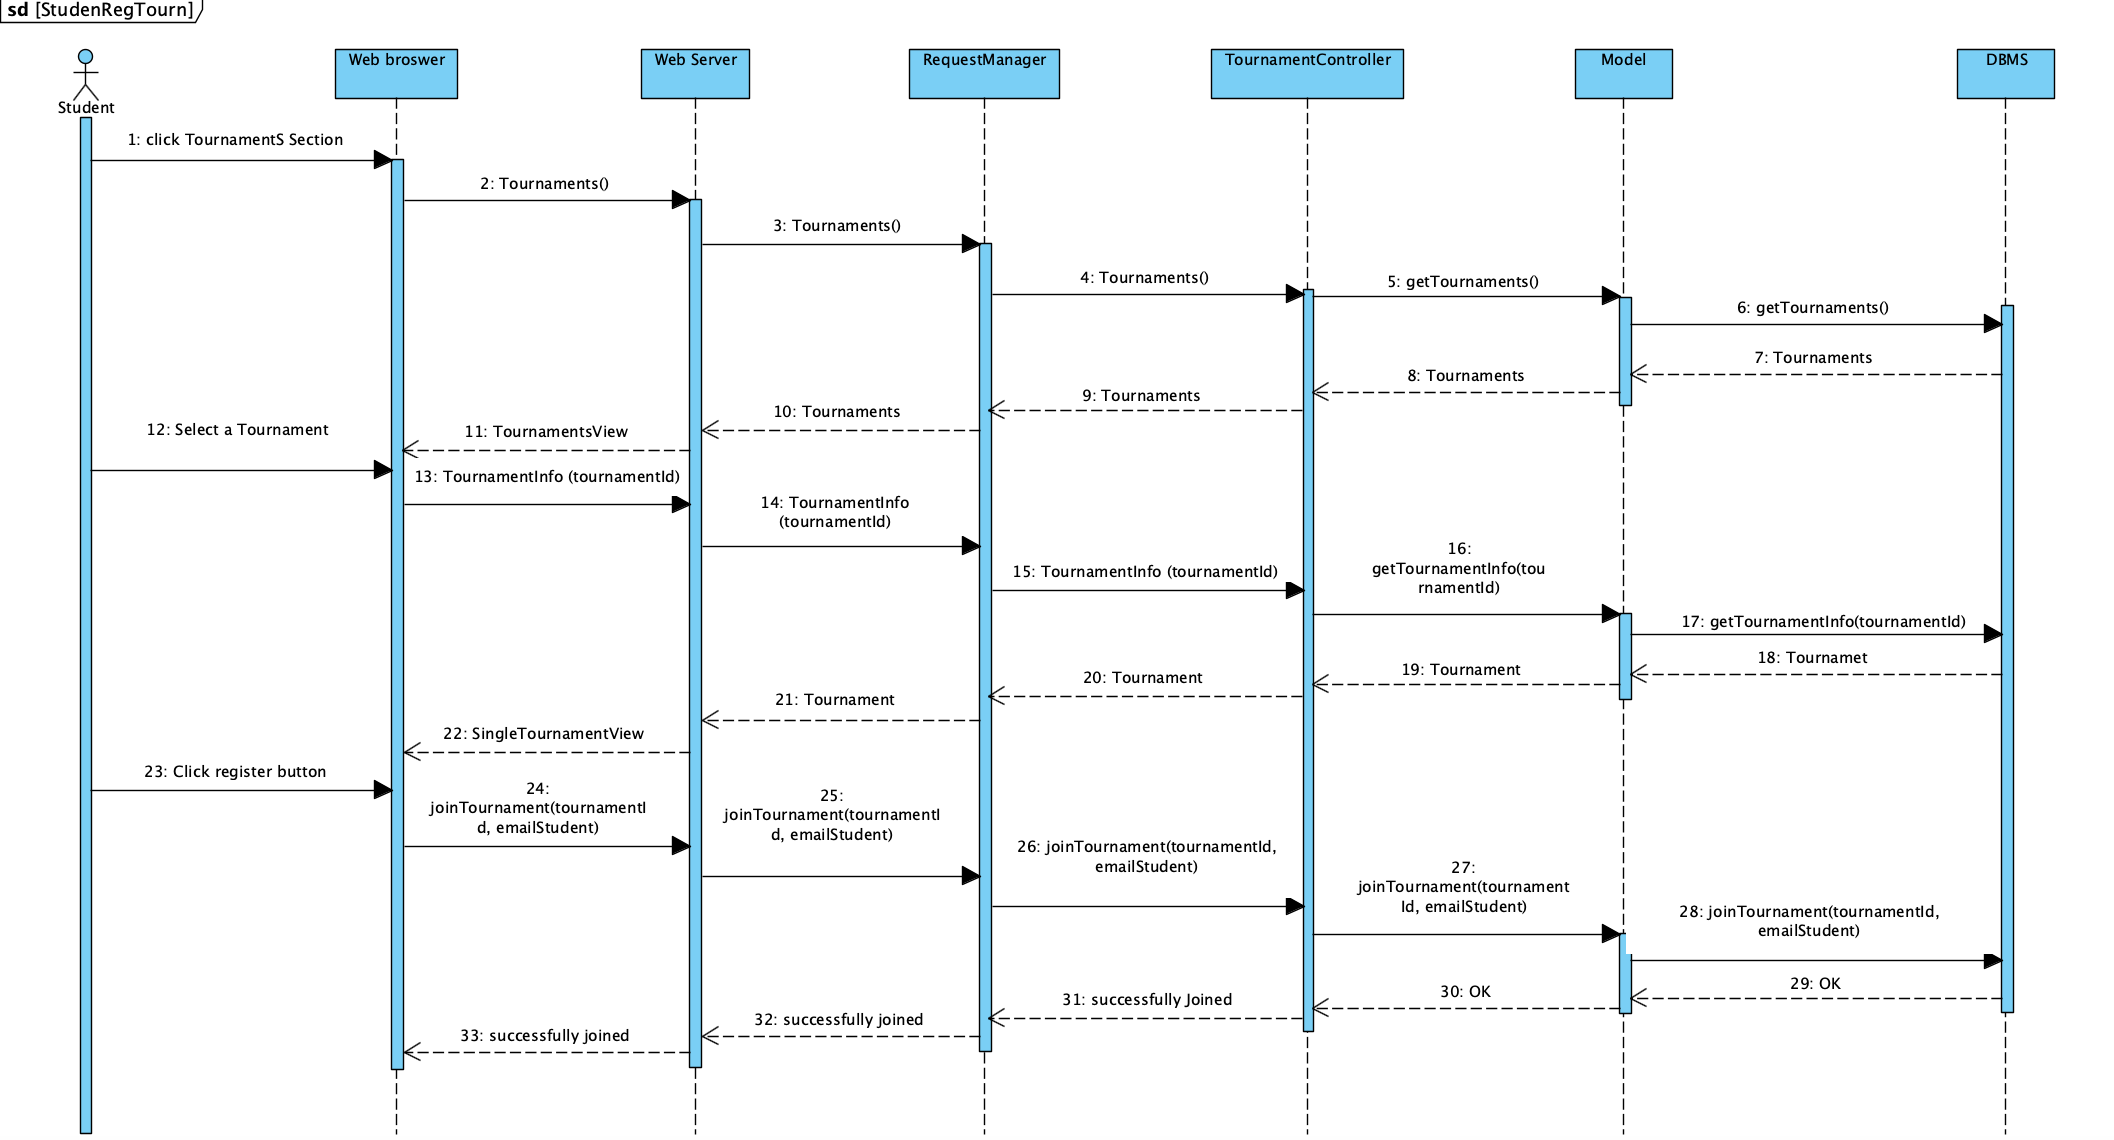
\includegraphics[width=1\textwidth]{SequenceDiagram/StudenRegTourn.png}
    \label{fig:enter-label}
\end{figure}
The sequence diagram describes the process of registering a student for a tournament through the  system. The student selects the "Tournaments" section from the dashboard, and the system displays a list of available tournaments. After browsing through the options, the student chooses a tournament of interest and the system presents the specific page of the selected tournament.
Once on the tournament page, the student initiates registration by clicking the "Register" button. This action triggers a series of events between the system components: the Web Browser transmits the request to the Web Server, which then passes the information to the Request Manager. The Request Manager coordinates the request with the Tournament Controller, which in turn requests the Model to retrieve and provide tournament information from the Database Management System (DBMS).
After displaying the tournament information, when the student confirms the registration, the Tournament Controller invokes the "joinTournament" function, which again interacts with the Model and the DBMS to register the student's participation in the tournament. The DBMS confirms the operation with an "OK", indicating that the registration has been successfully completed and that the student's data has been correctly updated in the database.
The process ends with the Web Browser confirming that the student has been successfully registered, and the student receives a message confirming their participation in the tournament.

\subsubsection{Student registers for the Battle}
\begin{figure}[H]
    \centering
    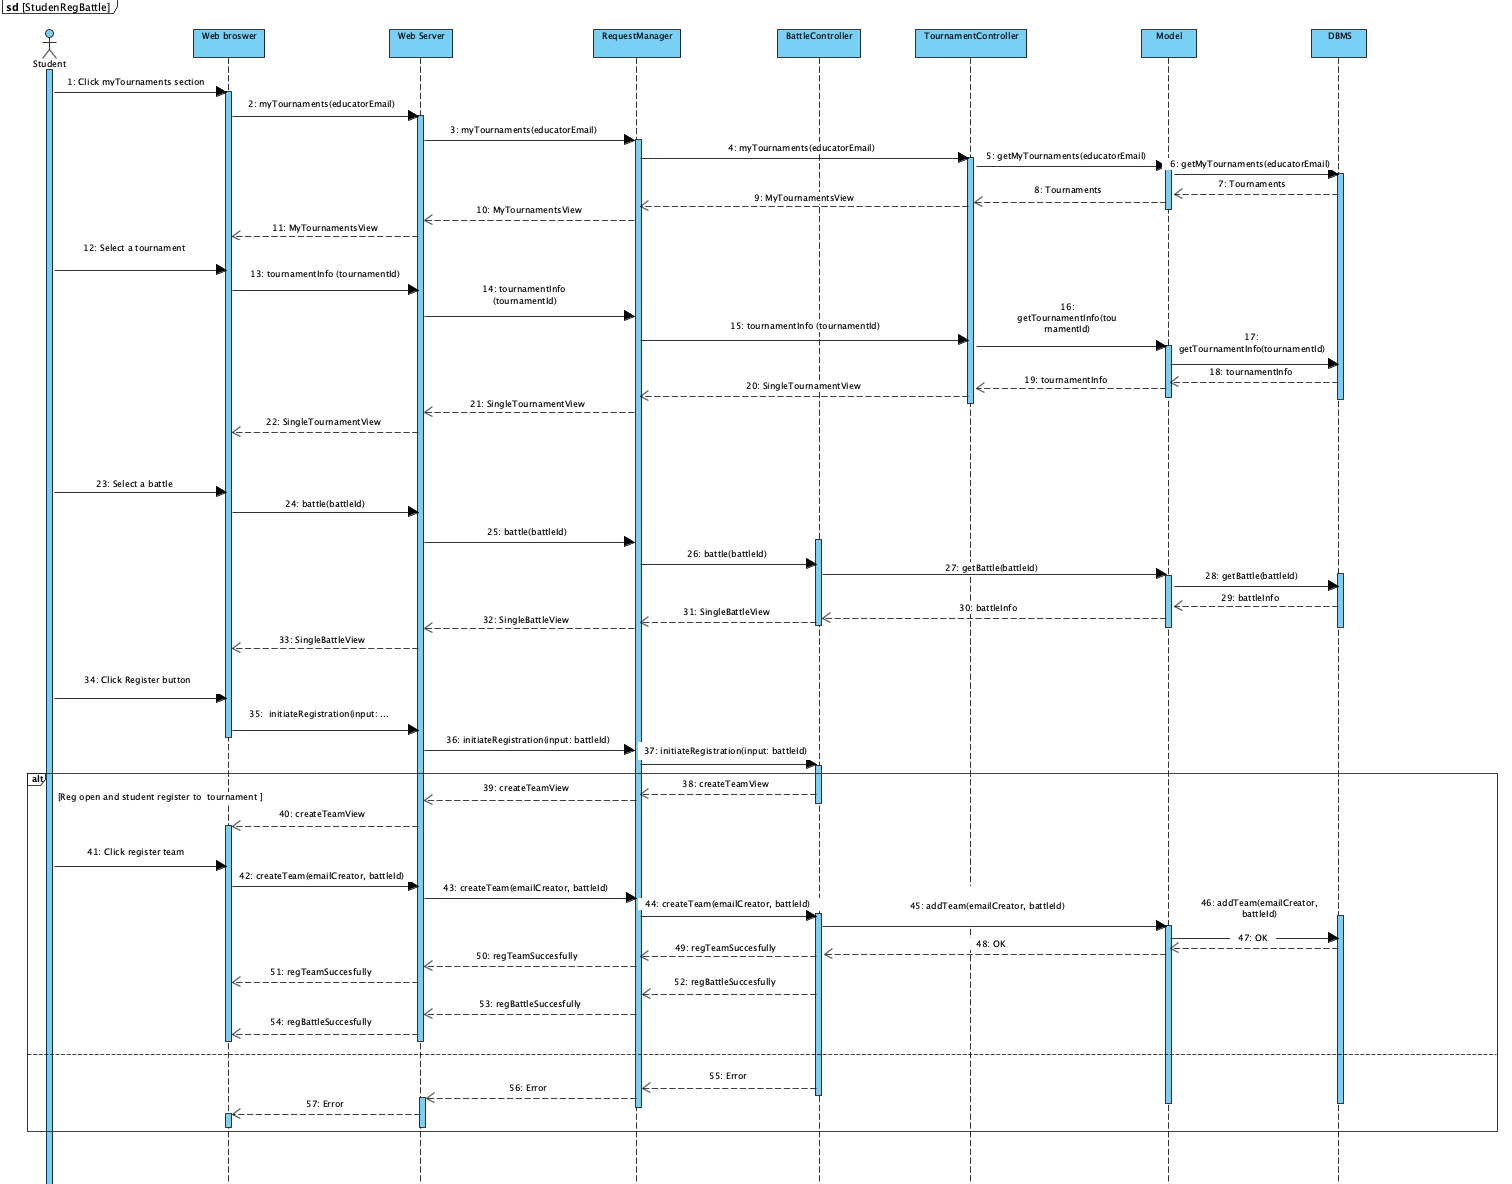
\includegraphics[width=1\textwidth]{SequenceDiagram/RegggBattle.png}
    \label{fig:enter-label}
\end{figure}
The sequence diagram describes the process of registering a student for a battle within a tournament. After selecting the desired tournament and battle from the Web Browser, the Request Manager directs the request to the Battle Controller for operations relating to the specific battle. The Battle Controller, in turn, queries the Model to obtain the details of the battle. The Model acts as an abstraction of the tournament data and facilitates interaction with the Database Management System (DBMS). This allows the student to view the details of the specific battle and press the register button. At this point, the student displays createTeamView in which they register their team by entering the necessary information. Once the DBMS has confirmed the addition of the data with an 'OK', the Battle Controller receives this confirmation and forwards the success information to the Request Manager. The Request Manager then informs the Web Server that the registration has been successfully completed. Finally, the Web Server communicates with the Web Browser, allowing the system to display a confirmation message to the student confirming the team's registration for the selected battle. If the registration for the battle is not open, or the student is not registered for the tournament of which the battle is a part, the student receives an error message.

\subsubsection{Student invites other students to create a Team}
\begin{figure}[H]
    \centering
    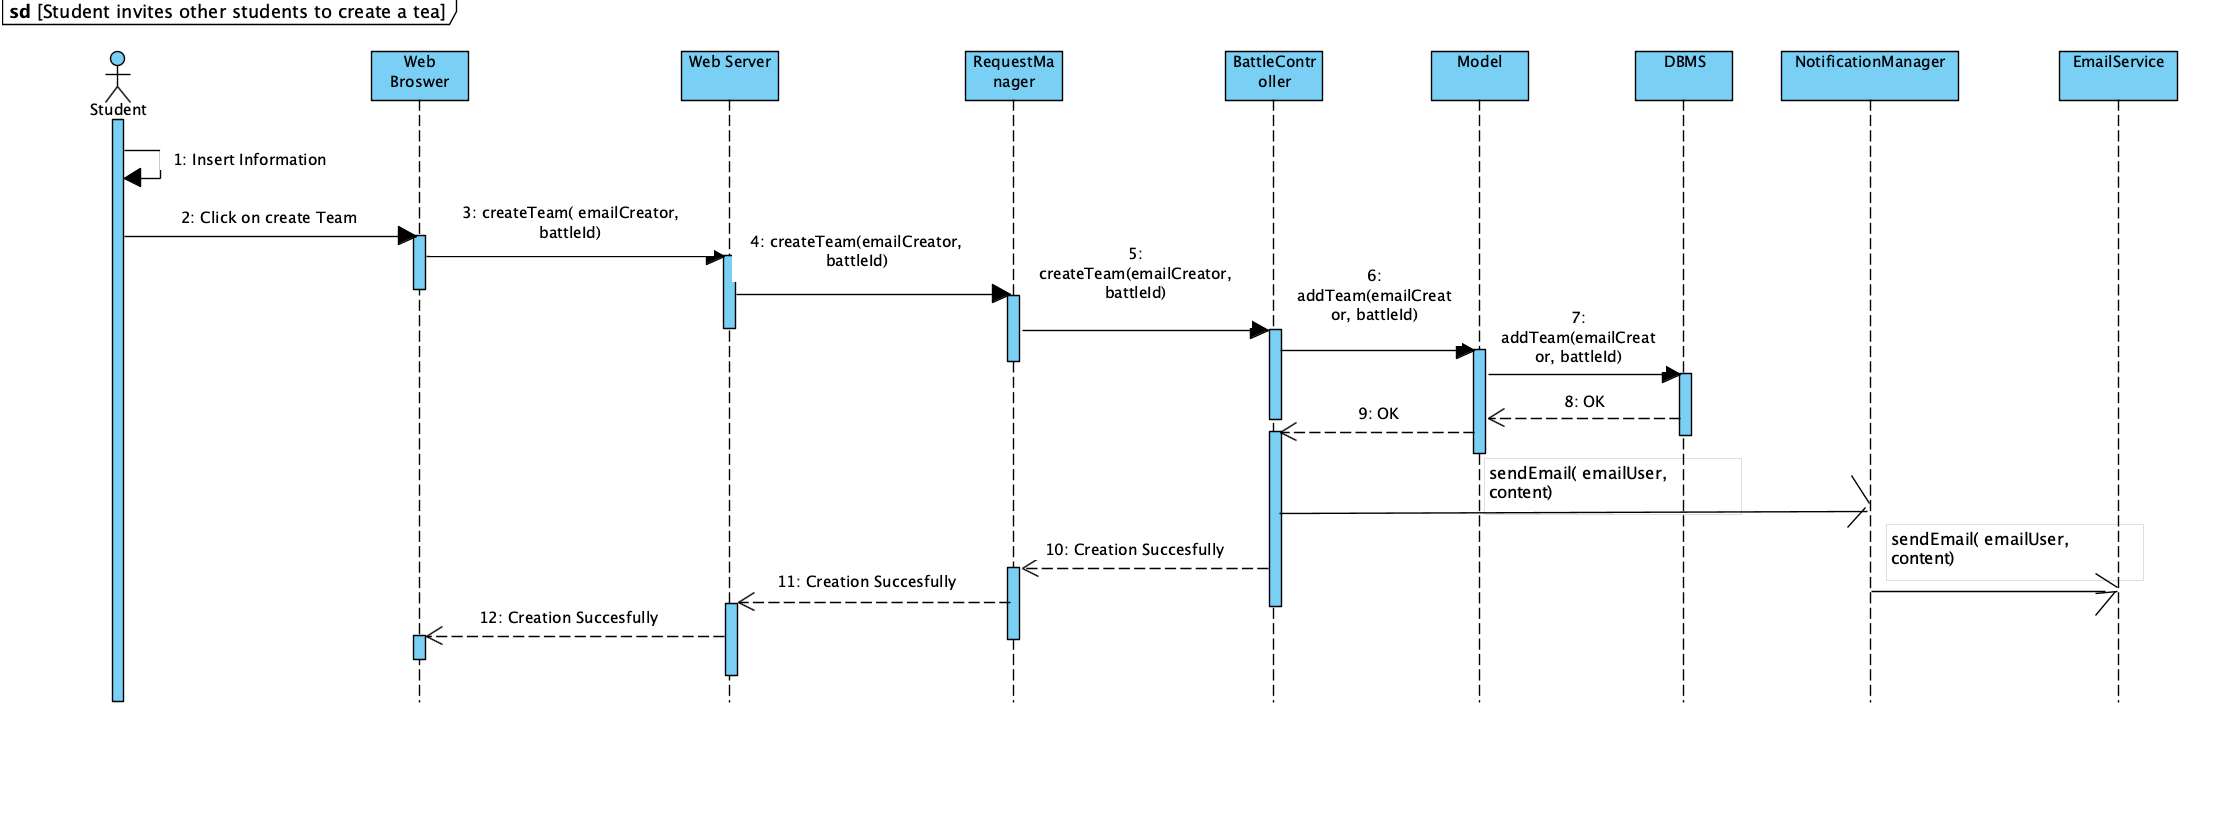
\includegraphics[width=1\textwidth]{SequenceDiagram/StudentsInviteOtherStudents.png}
    \label{fig:enter-label}
\end{figure}
The sequence diagram shows the flow of events for the formation of a team by a student within the platform. After selecting "Register" for a specific battle, the student enters the team name and selects the students to form the team.

The flow begins with the student entering the required information into the Web Browser. This information includes the team name and email addresses of the invited students. After entering this information, the student proceeds by clicking the "Create Team" button. The Web Browser sends the request to the Web Server, which passes the details to the Request Manager.  The Request Manager directs the request to the Battle Controller, which handles the business logic related to the formation of teams in battles. The Battle Controller invokes the Model to add the team to the system. The Model then interacts with the Database Management System (DBMS) to register the new team, associating the team name, battle identifier and email addresses of the invited students with the corresponding record.

Once the DBMS confirms the addition of the team with an "OK" response, indicating that the team has been successfully created in the database, the Notification Manager is activated. The Notification Manager coordinates with the Email service to send an email notification to all invited students, informing them of their inclusion in the team and providing relevant details.

The system then confirms the creation of the team to the student via the Web Browser, thus completing the process.

\subsubsection{Student accept invitations and become part of the Team}
\begin{figure}[H]
    \centering
    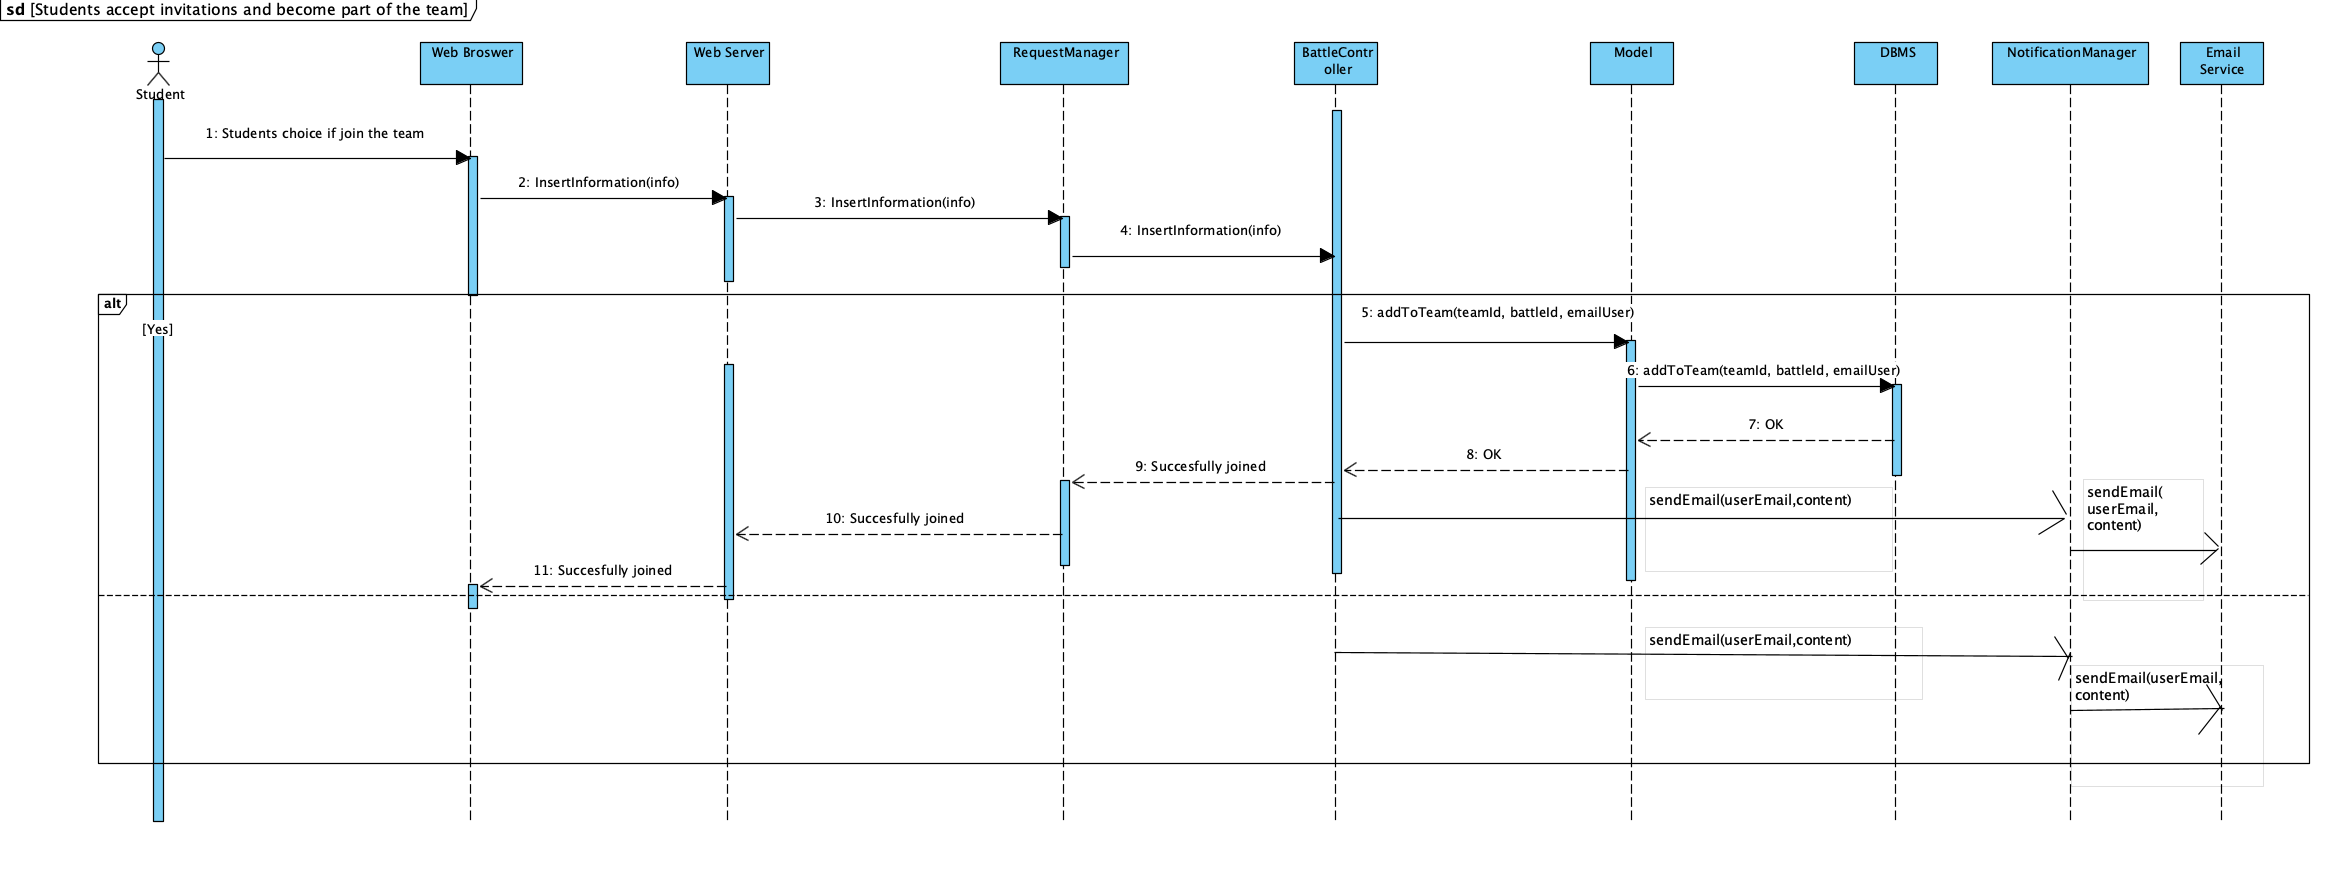
\includegraphics[width=1\textwidth]{SequenceDiagram/Students accept invitations and become part of the team.png}
    \label{fig:enter-label}
\end{figure}
The sequence diagram starts with the students receiving an email containing a link. When students click on the link, the Web Browser processes the request and directs them to the homepage of the platform (CKB). Once the system displays the confirmation message, students can choose to accept the invitation by clicking 'Yes'.
At this point, the Web Server receives an indication of acceptance of the invitation and passes this information to the Request Manager. The Request Manager acts as coordinator of the data flow, ensuring that the request is correctly addressed.
It then transfers the team membership request to the Battle Controller. The Battle Controller invokes the Model to make the change in the system, adding the user to the specific team.
The Model interfaces with the DBMS to update the team record with the new members. The DBMS performs the update operation and, once the transaction is confirmed with an 'OK', the Model notifies the Battle Controller that the addition has been successfully completed.
After the Battle Controller has received the confirmation, the Notification Manager is activated to handle the notification of users. The Notification Manager makes use of the Email service to send an email notification to all team members, confirming their team membership.
If the student declines the invitation, only the team creator is notified.
\subsubsection{Battle Setup}
\begin{figure}[H]
    \centering
    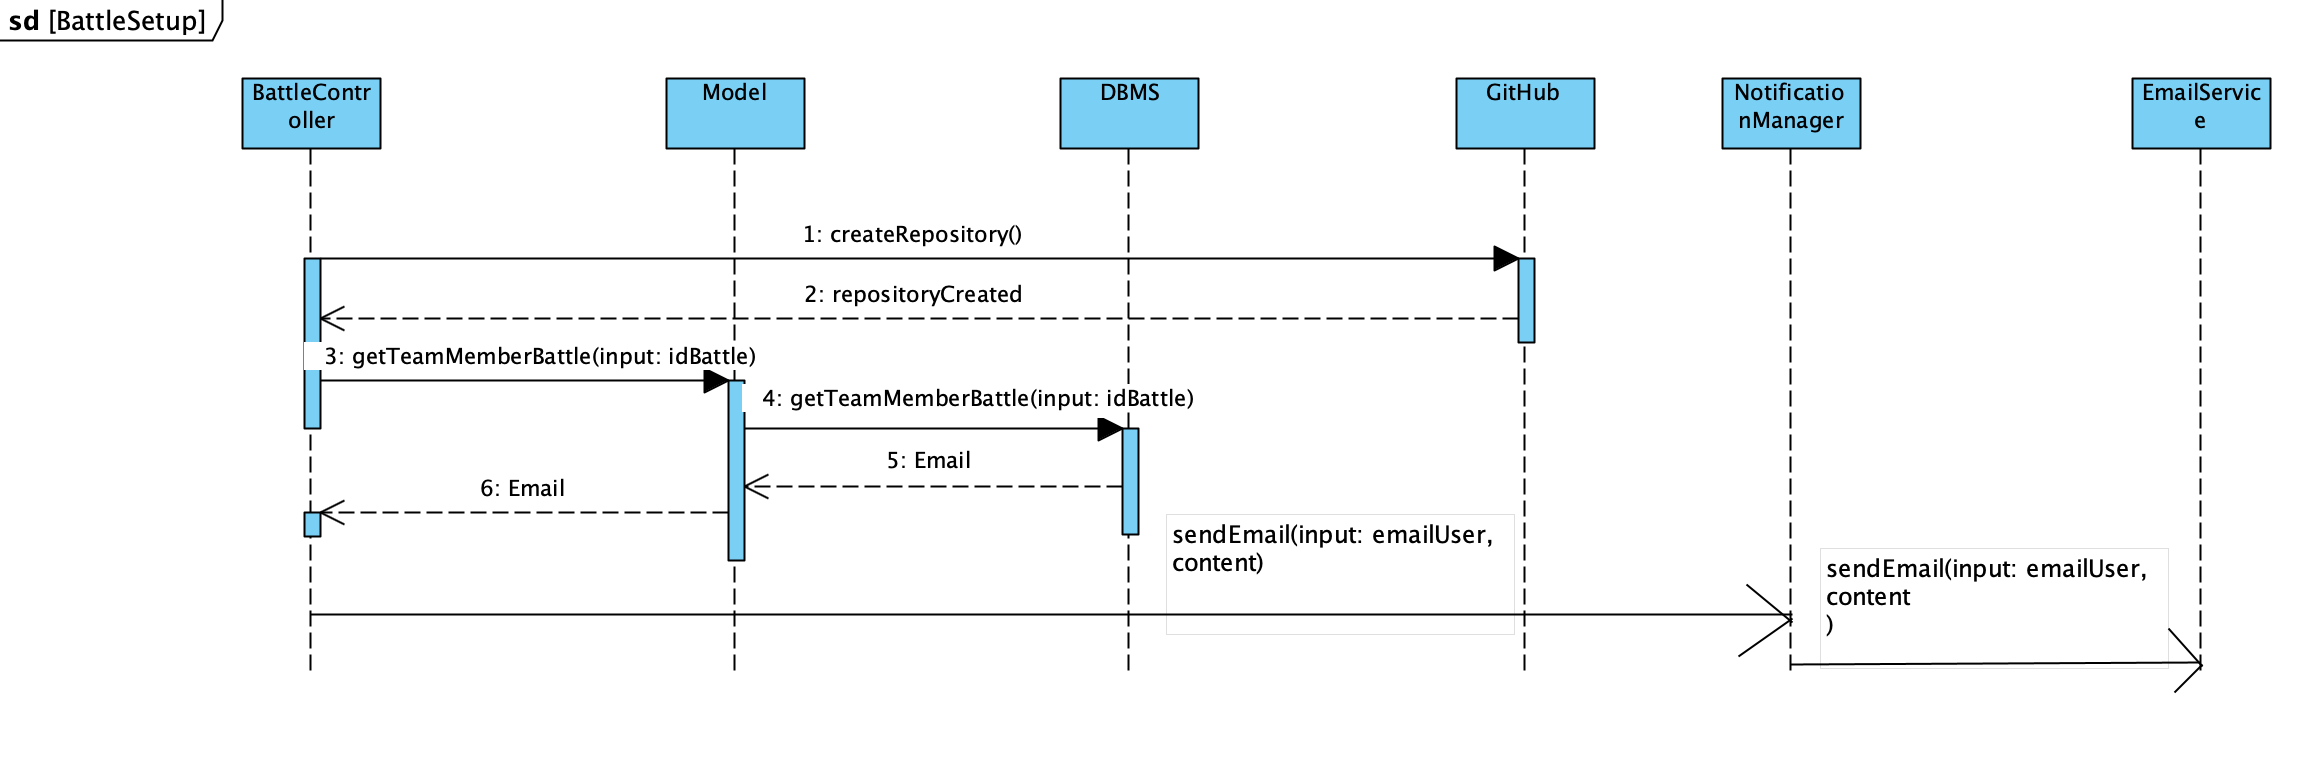
\includegraphics[width=1\textwidth]{SequenceDiagram/BattleSetup.png}
    \label{fig:enter-label}
\end{figure}
The sequence diagram illustrates the process of setting up the environment for a coding battle after the registration deadline.
Once registration is closed, the platform proceeds with the creation of a GitHub repository to contain the code kata, i.e. the project on which the students will work. This is managed by the Battle Controller, which invokes the CreateRepository() function on the GitHub component.
Once the repository has been created, the BattleController retrieves all the emails of the participants in the battle and via the NotificationManager sends an email to all students. This email contains the link to the GitHub repository and instructions for setting up an automated workflow using GitHub Actions. The Notification Manager relies on the Email service to send these details to the students.
 

\subsubsection{Student start to work}
\begin{figure}[H]
    \centering
    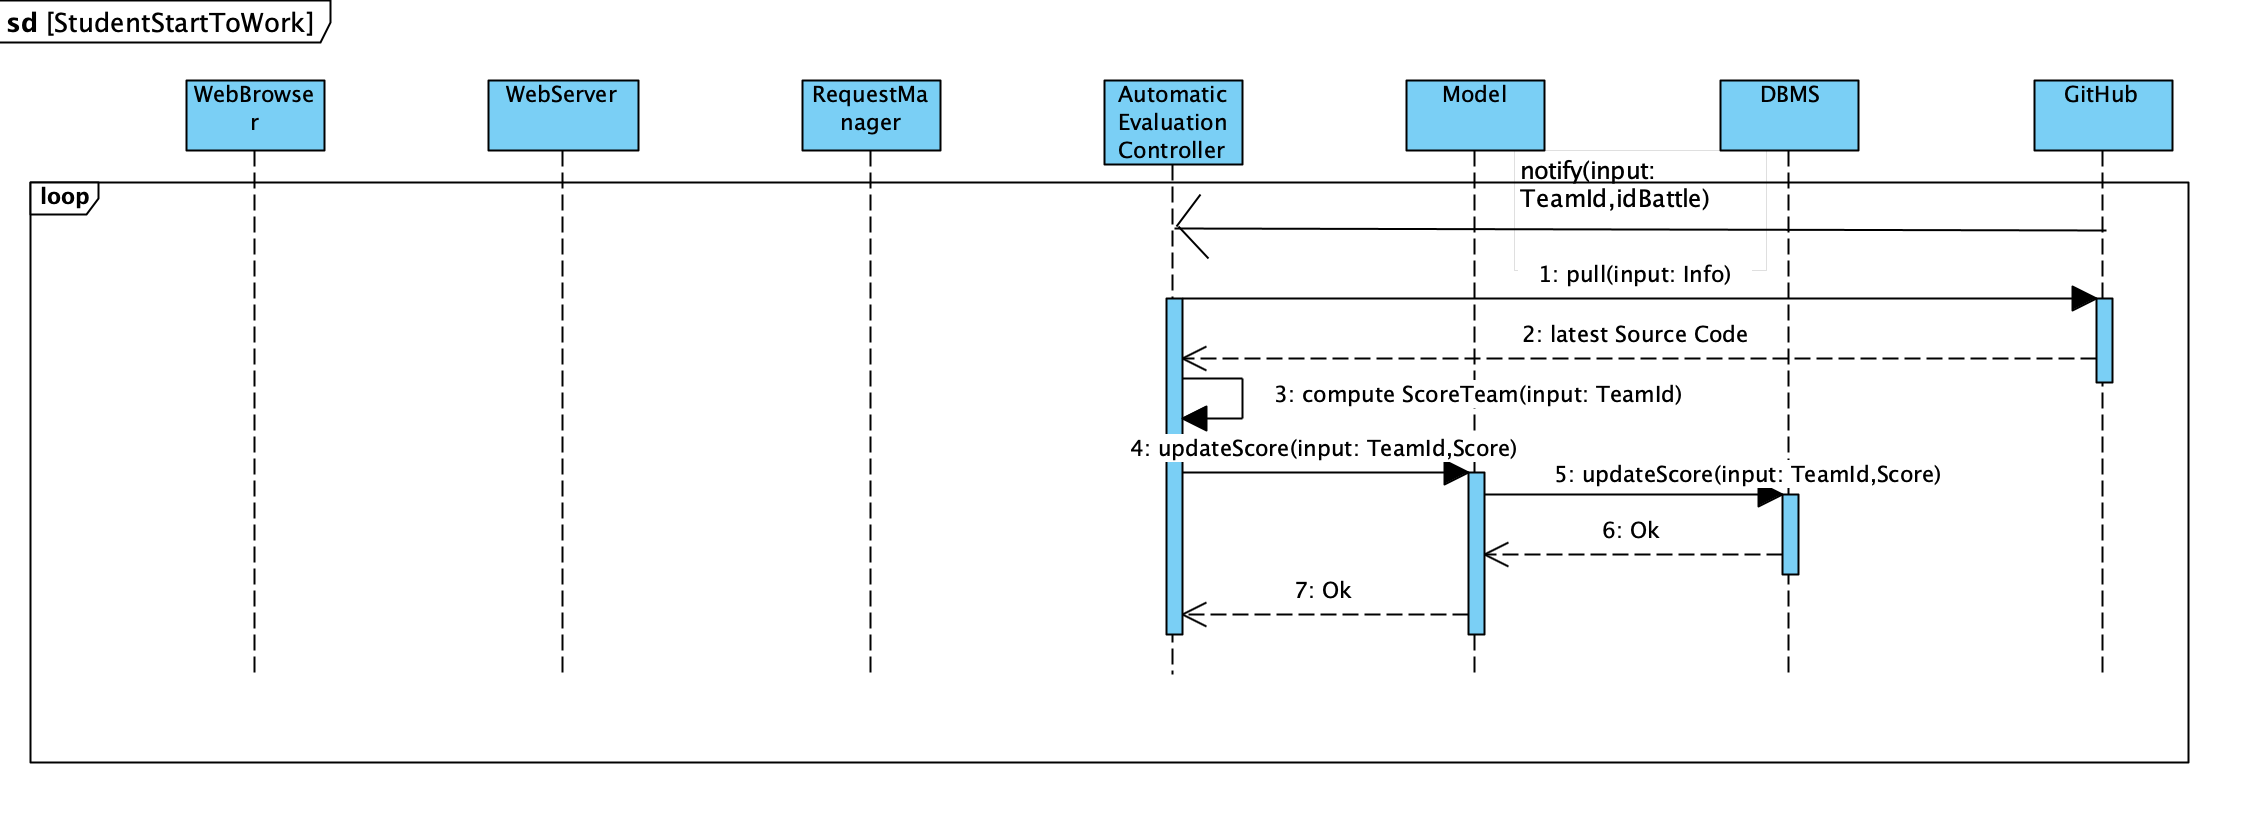
\includegraphics[width=1\textwidth]{SequenceDiagram/StudentStartToWork.png}
    \label{fig:enter-label}
\end{figure}
The sequence diagram describes the operations performed once the battle environment has been successfully configured and the students begin work.
The students start working on the code within the GitHub repository dedicated to the project. As they develop their work, they commit to GitHub for each significant update they want to save and share. This is a continuous and iterative process, as indicated by the 'loop' element in the diagram.
When a new commit is made, the GitHub component, which was configured during the battle setup phase, sends a notification to the CKB platform. These notifications are a signal that there are new changes to be evaluated.
Upon receiving notification of a new commit, the CKB system, through the AutomaticEvaluationController, interacts with the Model to 'pull' the latest changes from the GitHub repository. The Model then requests the Database Management System (DBMS) to update the latest data, thus keeping the project status synchronised with the latest student submissions.
Immediately afterwards, the system proceeds with the calculation of the team score. Once the score has been calculated, the model updates the DBMS with the new team score.
Finally, when the submission deadline is reached, the system stops monitoring further code pushes. This moment marks the end of the battle.



\subsubsection{Educator evaluation during the consolidation process}
\begin{figure}[H]
    \centering
    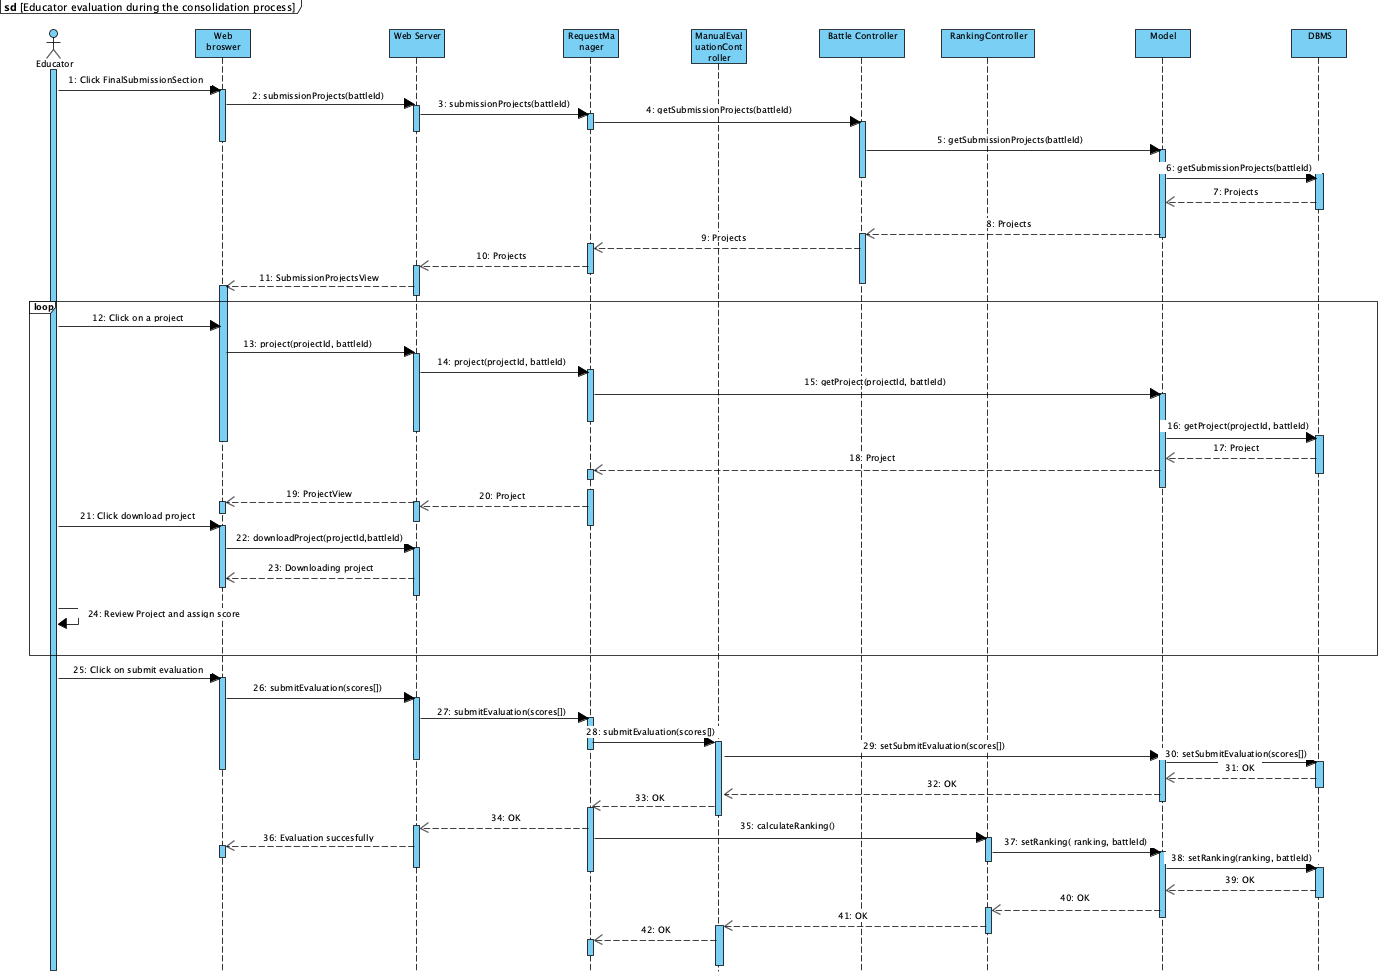
\includegraphics[width=1\textwidth]{SequenceDiagram/ConsProcc.png}
    \label{fig:enter-label}
\end{figure}
The sequence diagram reflects the evaluation process an educator follows after the deadline for project submissions has ended in a battle. The educator accesses the platform through his or her browser and selects the 'Final Submission' section to view the students' final submissions. This action is recorded by the Web Server, which communicates with the Request Manager, which in turn interacts with the Manual Evaluation Controller.
The Manual Evaluation Controller requests the Model to retrieve projects from the Database Management System. These projects are then presented to the educator, who can click on each one to examine the details. For each project, the educator has the option of downloading the corresponding files, examining them and assigning a score based on his or her evaluation. When the educator enters all the evaluations (loops), they are sent by the educator via the web browser, to the Web Server, then to the Request Manager and finally to the Manual Evaluation Controller, which updates the database with the new scores via the Model.
Once the evaluation of all projects is complete, the Ranking Controller comes into play. This component processes the final scores, combining the educator's manual evaluations with those generated through automated processes. The final results are saved in the database and, through the Notification Manager, an email notification is sent to all participating students, providing them with ranking information that is now available.
%%%%%%%%%%%%%%%%%%%%%%%%%%%%%%%%%%%
\subsubsection{Educator monitors battle ranking}
\begin{figure}[H]
    \centering
    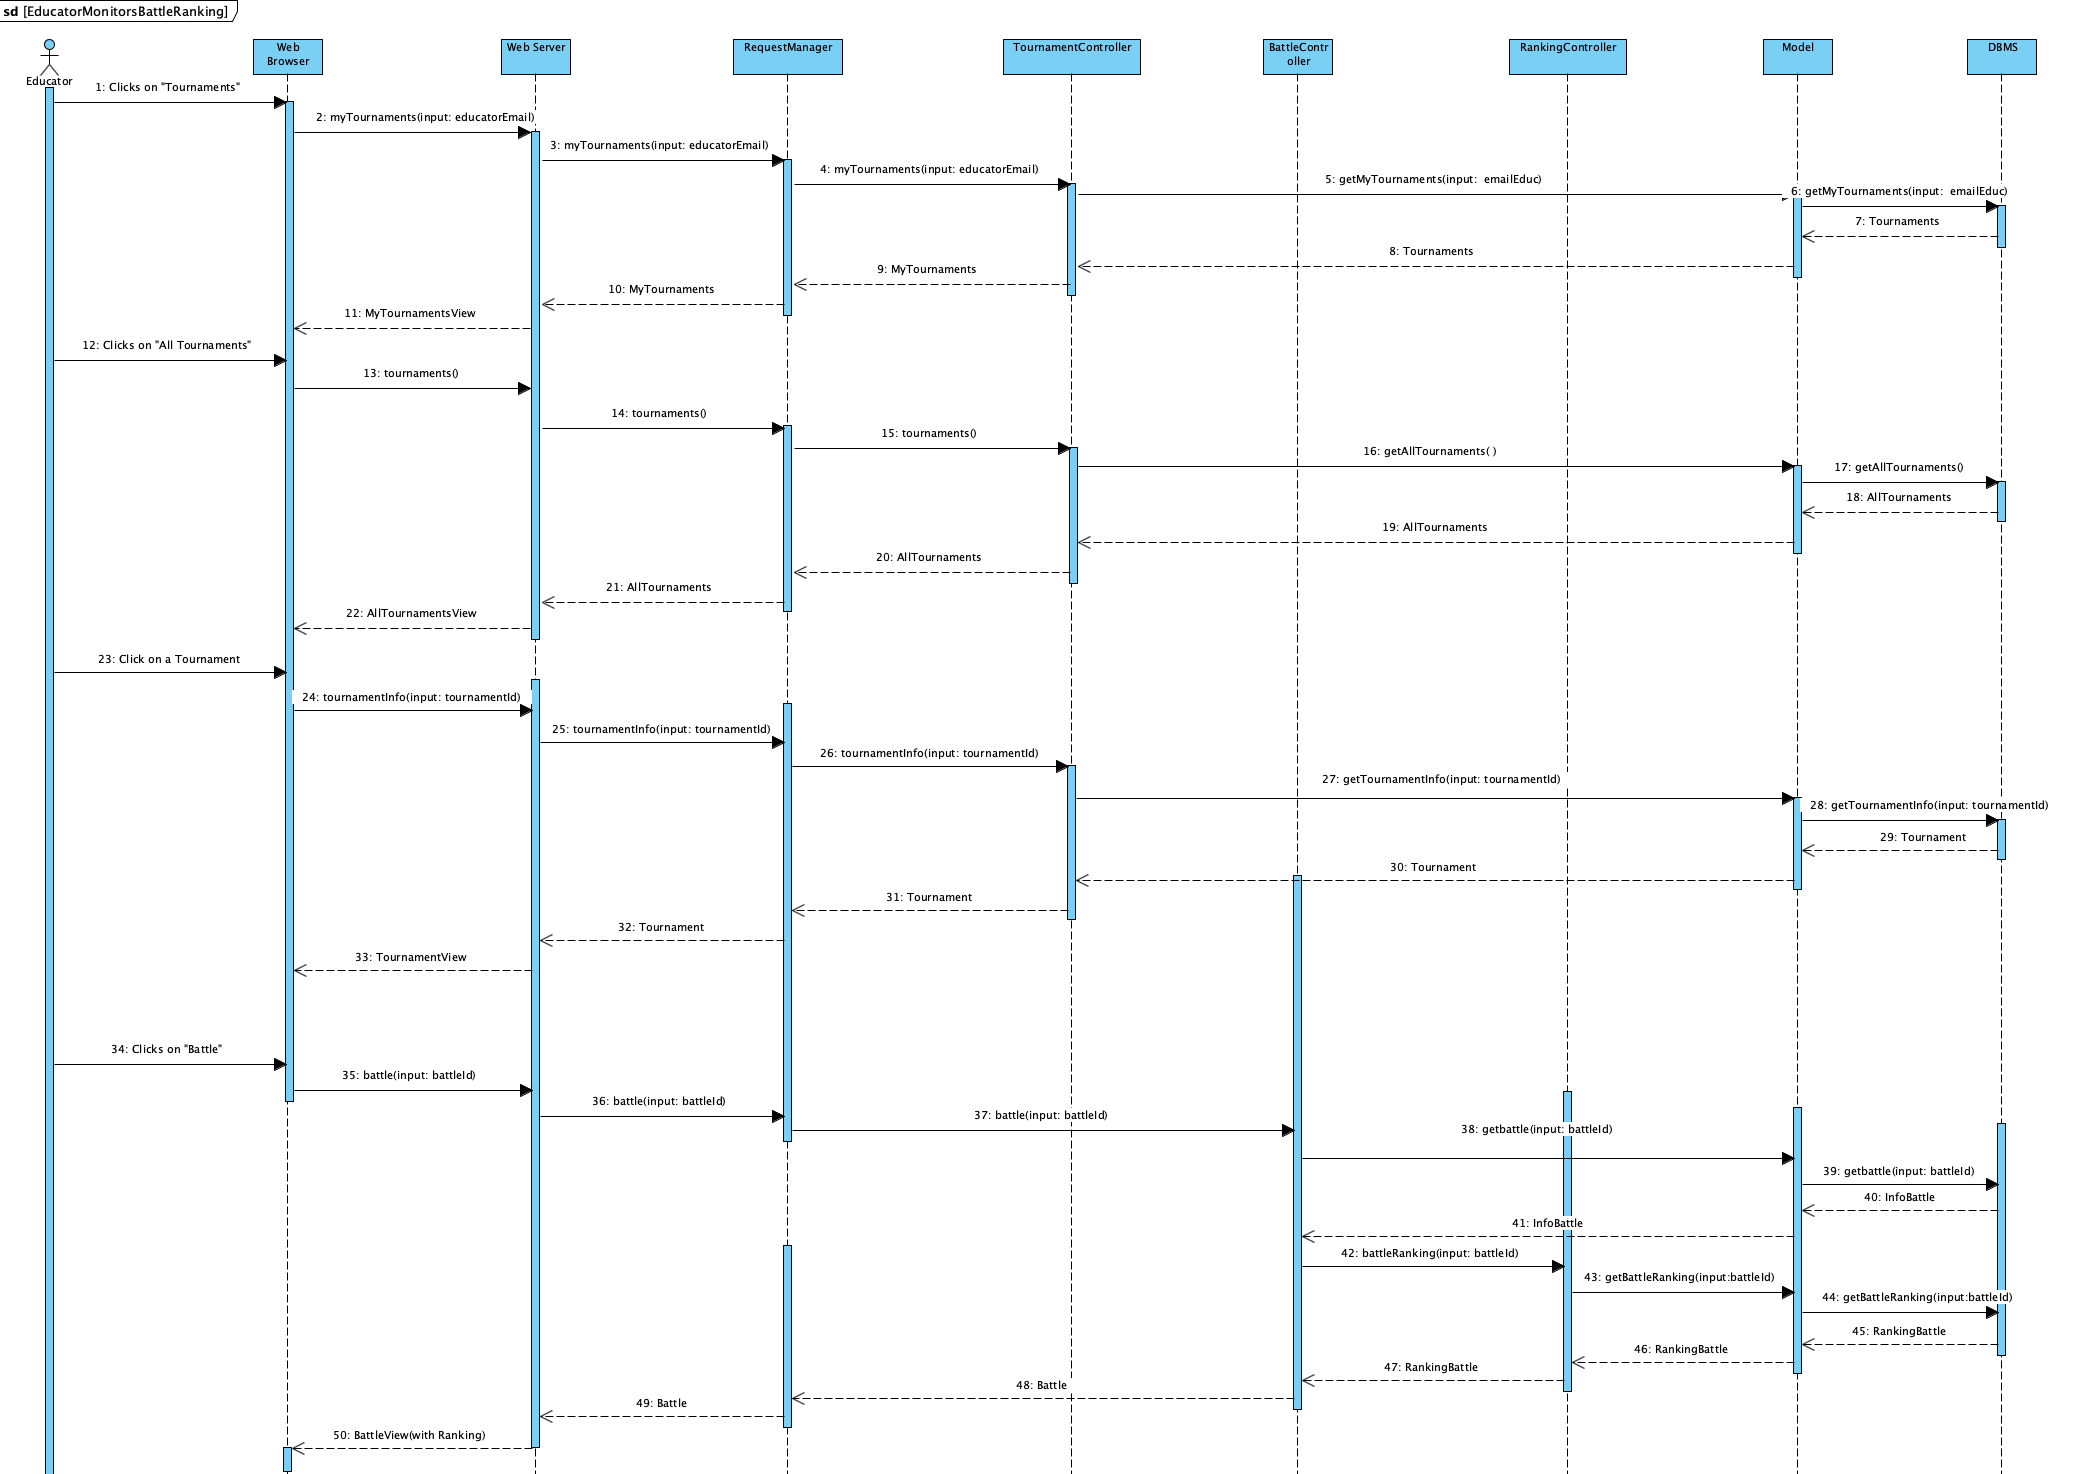
\includegraphics[width=1\textwidth]{SequenceDiagram/EducatorMonitorsBattleRanking.png}
    \label{fig:enter-label}
\end{figure}
In the sequence diagram, when the educator navigates through the platform to monitor the rankings, he initiates a series of interactions between various system components. After selecting the tournament section, his web browser sends a request to the web server, which is the entry point for all incoming requests. The web server passes the request to the Request Manager, which is routed to the Tournament Controller. This controller specialises in handling tournament-related operations. When the educator chooses a tournament and then a specific battle to display the rankings, the Tournament Controller and the Battle Controller requests the Model to retrieve the relevant information from the Database Management System (DBMS). The DBMS performs the necessary operations to extract the required data and returns it to the Model. The Model then passes this information to the Ranking Controller, which is responsible for managing the rankings based on the criteria defined for the tournament. 
The ranking controller retrieves the rankings and, via the other components, presents them to the educator.


%%%%%%%%%%%%%%%%%%%%%%%%%%%%%%
\subsubsection{Student monitors battle ranking}
\begin{figure}[H]
    \centering
    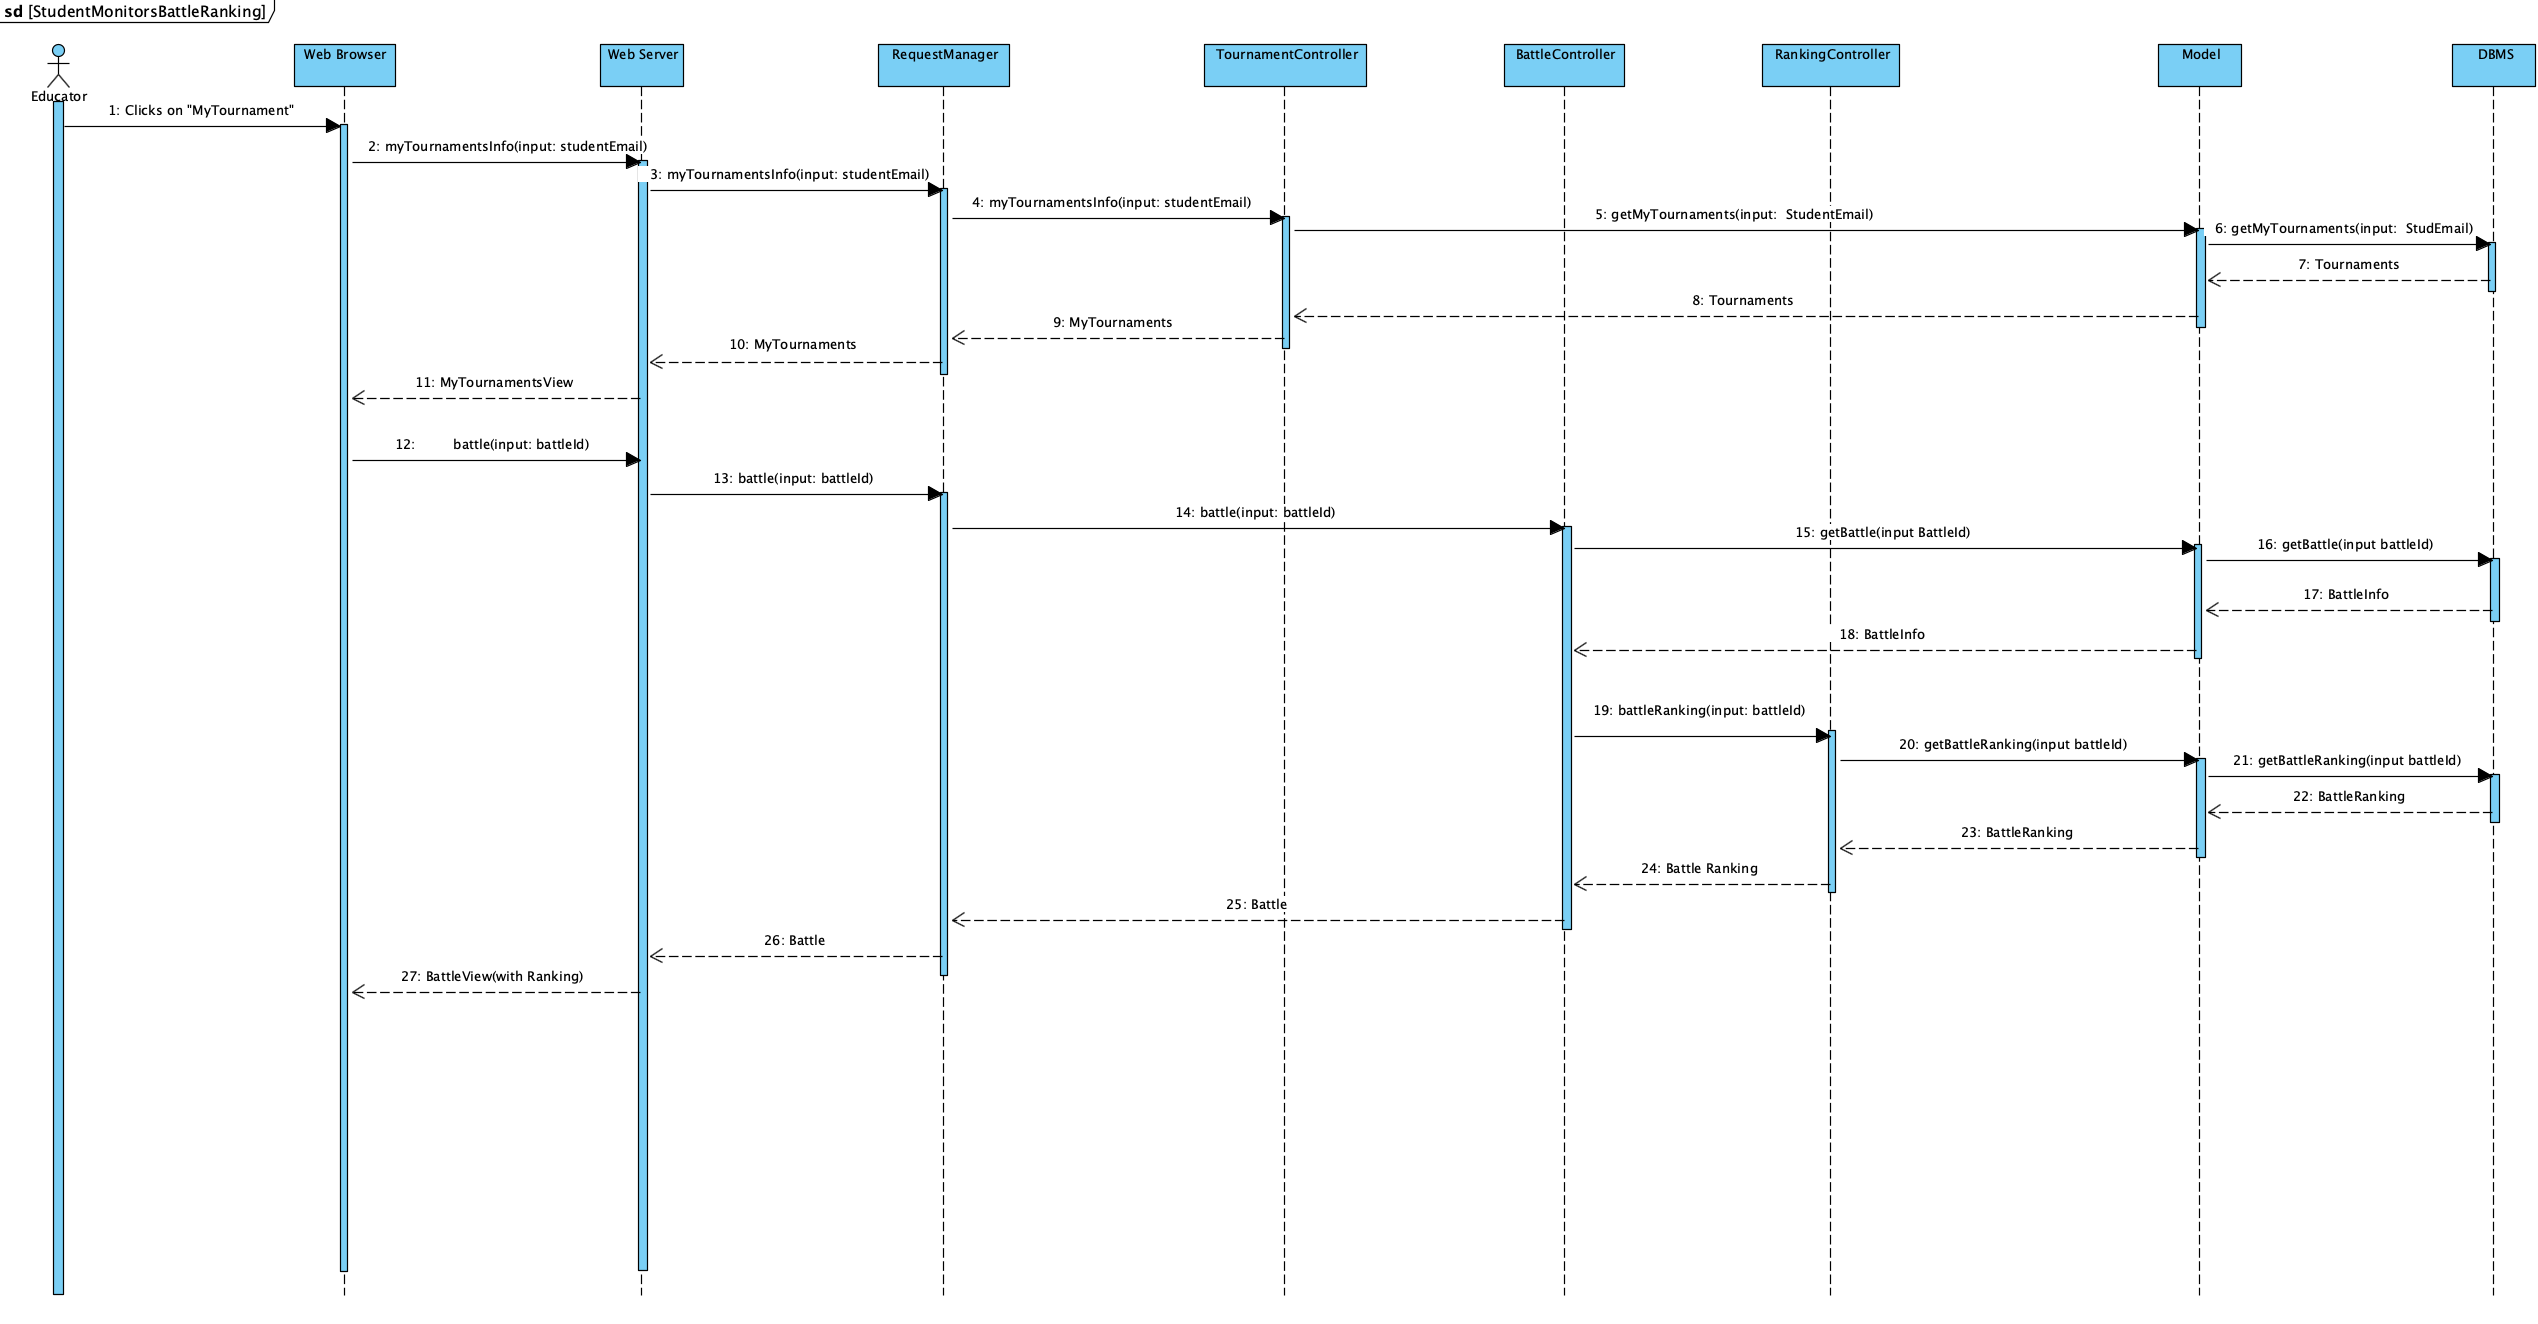
\includegraphics[width=1\textwidth]{SequenceDiagram/StudentMonitorsBattleRanking.png}
    \label{fig:enter-label}
\end{figure}
The sequence diagram illustrates how a student can access and view the ranking of a battle within a tournament via an online platform. Starting on the homepage, the student selects the "Tournaments" section, where the web server receives and forwards the request to the Request Manager. This, in turn, directs the request to the Tournament Controller.
The Tournament Controller is responsible for managing the tournament information. When the student selects a tournament, the Tournament Controller requests the Model to retrieve all information about the selected tournament from the DBMS, including the list of associated battles. The DBMS responds with the requested data, which the Model passes to the Tournament Controller, who then presents it to the student via the platform.
Next, the student selects a specific battle to view the ranking. At this point, the Battle Controller goes into action, retrieving the detailed information of the individual battle, again through the Model and the DBMS. 
Once the battle information has been retrieved, the Ranking Controller processes the data to generate a rankings display for the student to view. 
Eventually, the system presents the battle rankings to the student.
%%%%%%%%%%%%%%%%%%%%%%%%%%%%%%%%%%%%%%%%%%%%%%%%%
\subsubsection{Educator monitors tournament ranking}
\begin{figure}[H]
    \centering
    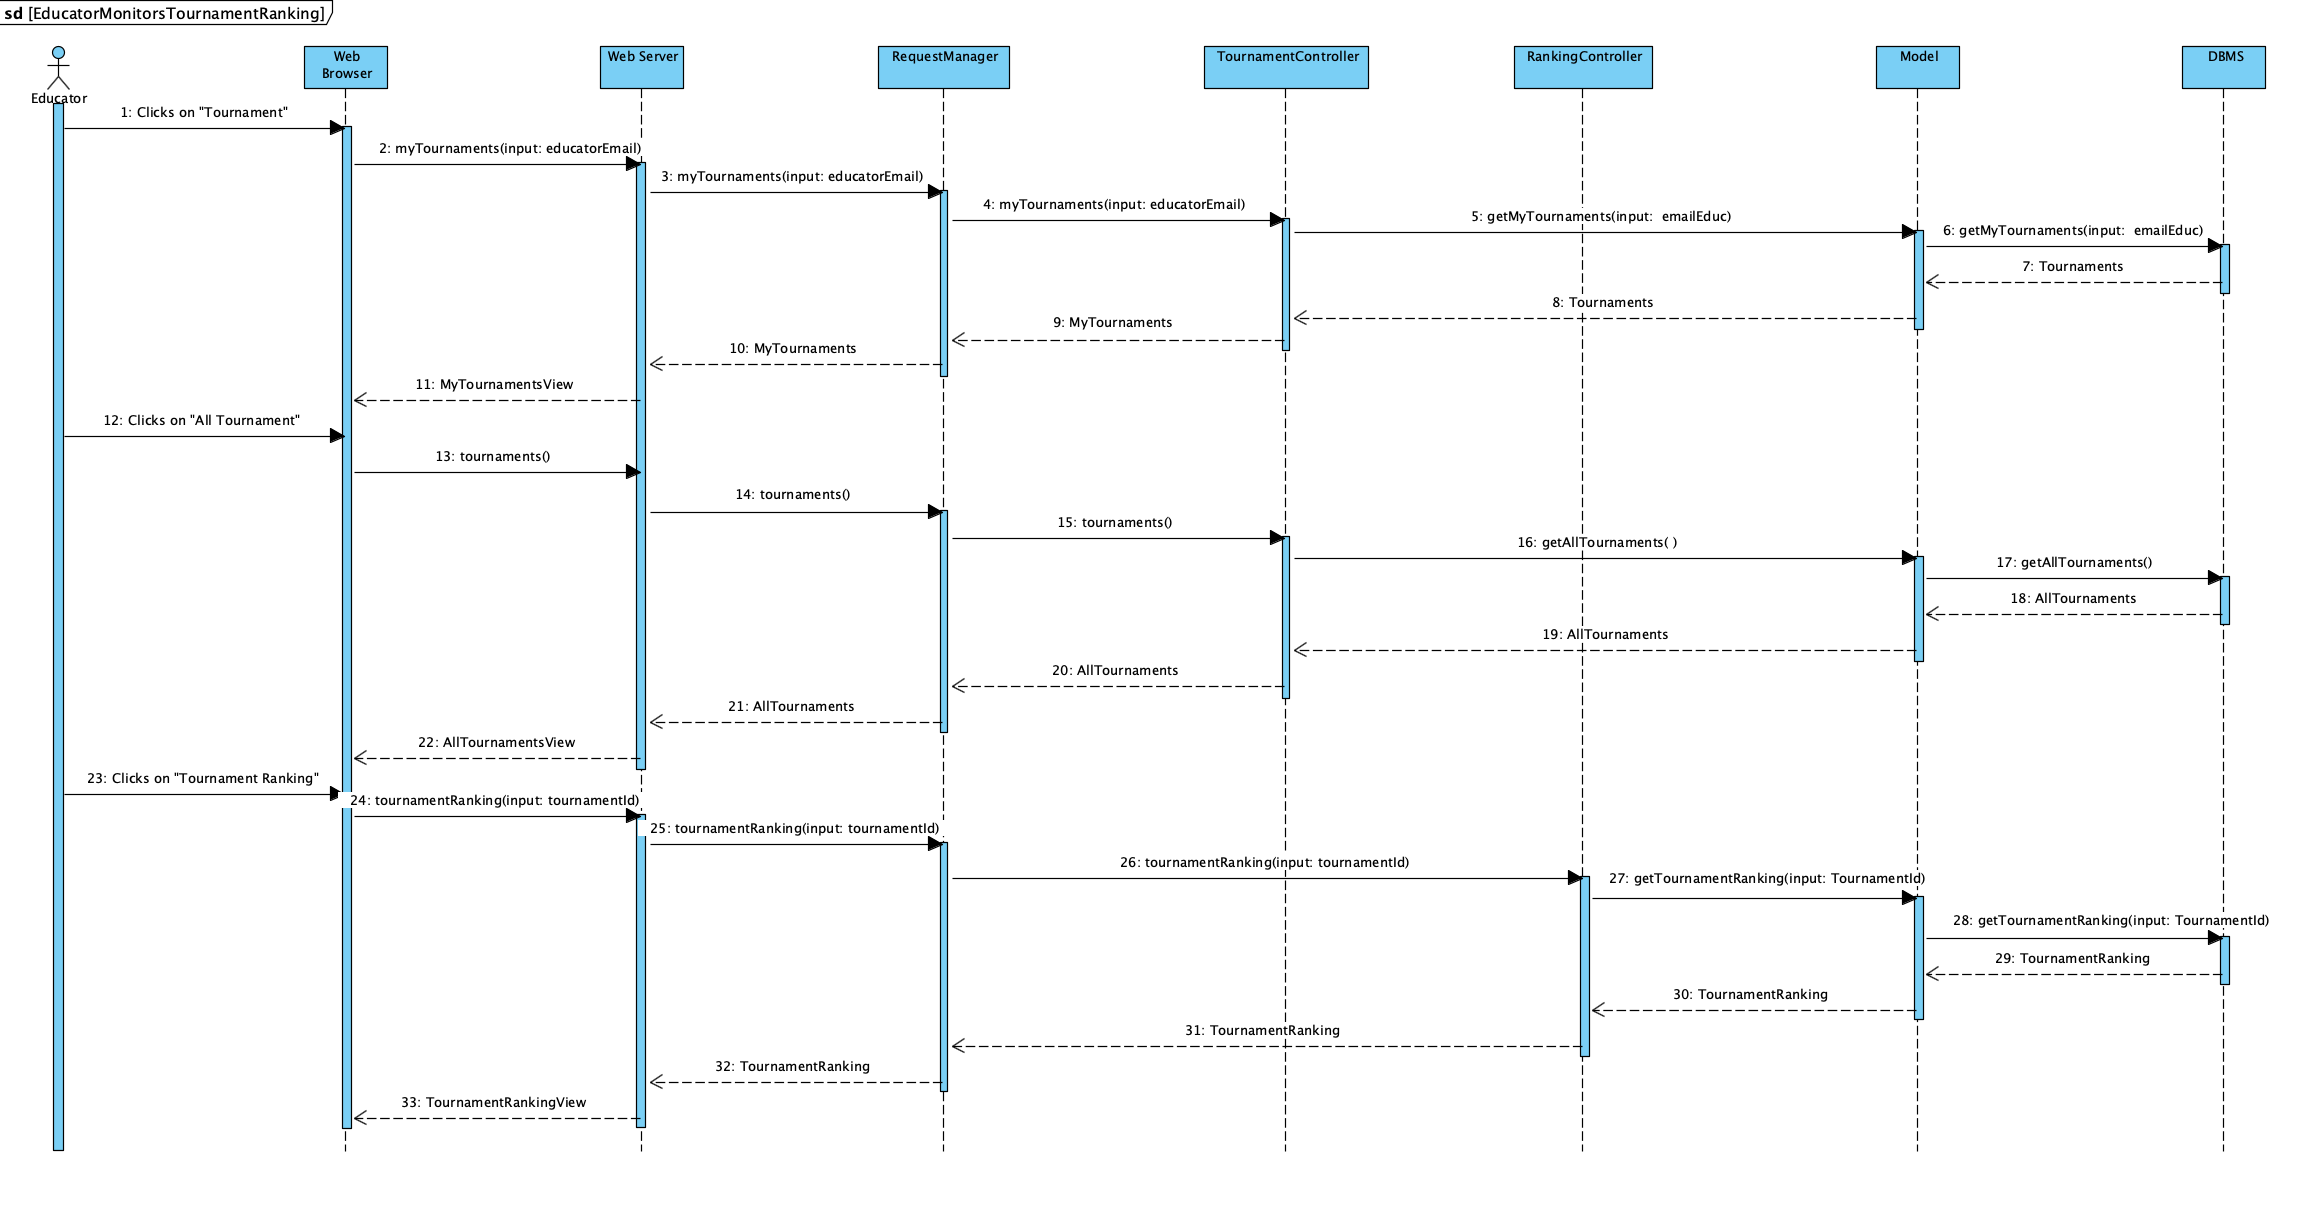
\includegraphics[width=1\textwidth]{SequenceDiagram/EducatorMonitorsTournamentRanking.png}
    \label{fig:enter-label}
\end{figure}
In the sequence diagram, an educator follows a series of steps on the online platform to view the ranking of a tournament. Starting from the homepage, the educator accesses the 'Tournaments' section, which shows him/her a control dashboard. This dashboard provides an overview of the tournaments the educator has created or for which he/she has permission to organise battles.
After clicking on 'All Tournaments', the system displays a page listing all tournaments available on the platform, including those to which the educator cannot make changes. The educator then selects a specific tournament from the list. In response, the system displays a new dashboard detailing the battles associated with that tournament, also providing the option to view the tournament leaderboard.
When the educator clicks on the "Tournament Rankings" button, the system processes a request to view the rankings for the selected tournament. This request is sent from the web browser to the web server, then passed through the Request Manager, which directs the request to the Ranking Controller.
The Ranking Controller, in turn, interacts with the Model to query the Database Management System (DBMS) for ranking data. The Model retrieves this information and passes it back to the Ranking Controller.  The latter passes the ranking view to the RequestManager which passes it to the Web Server until it reaches the Web Browser where the educator displays the tournament ranking.
%%%%%%%%%%%%%%%%%%%%%%%%%%%%%%%%%%%%%%%%%%%%%%%%%
\subsubsection{Student monitors tournament ranking}
\begin{figure}[H]
    \centering
    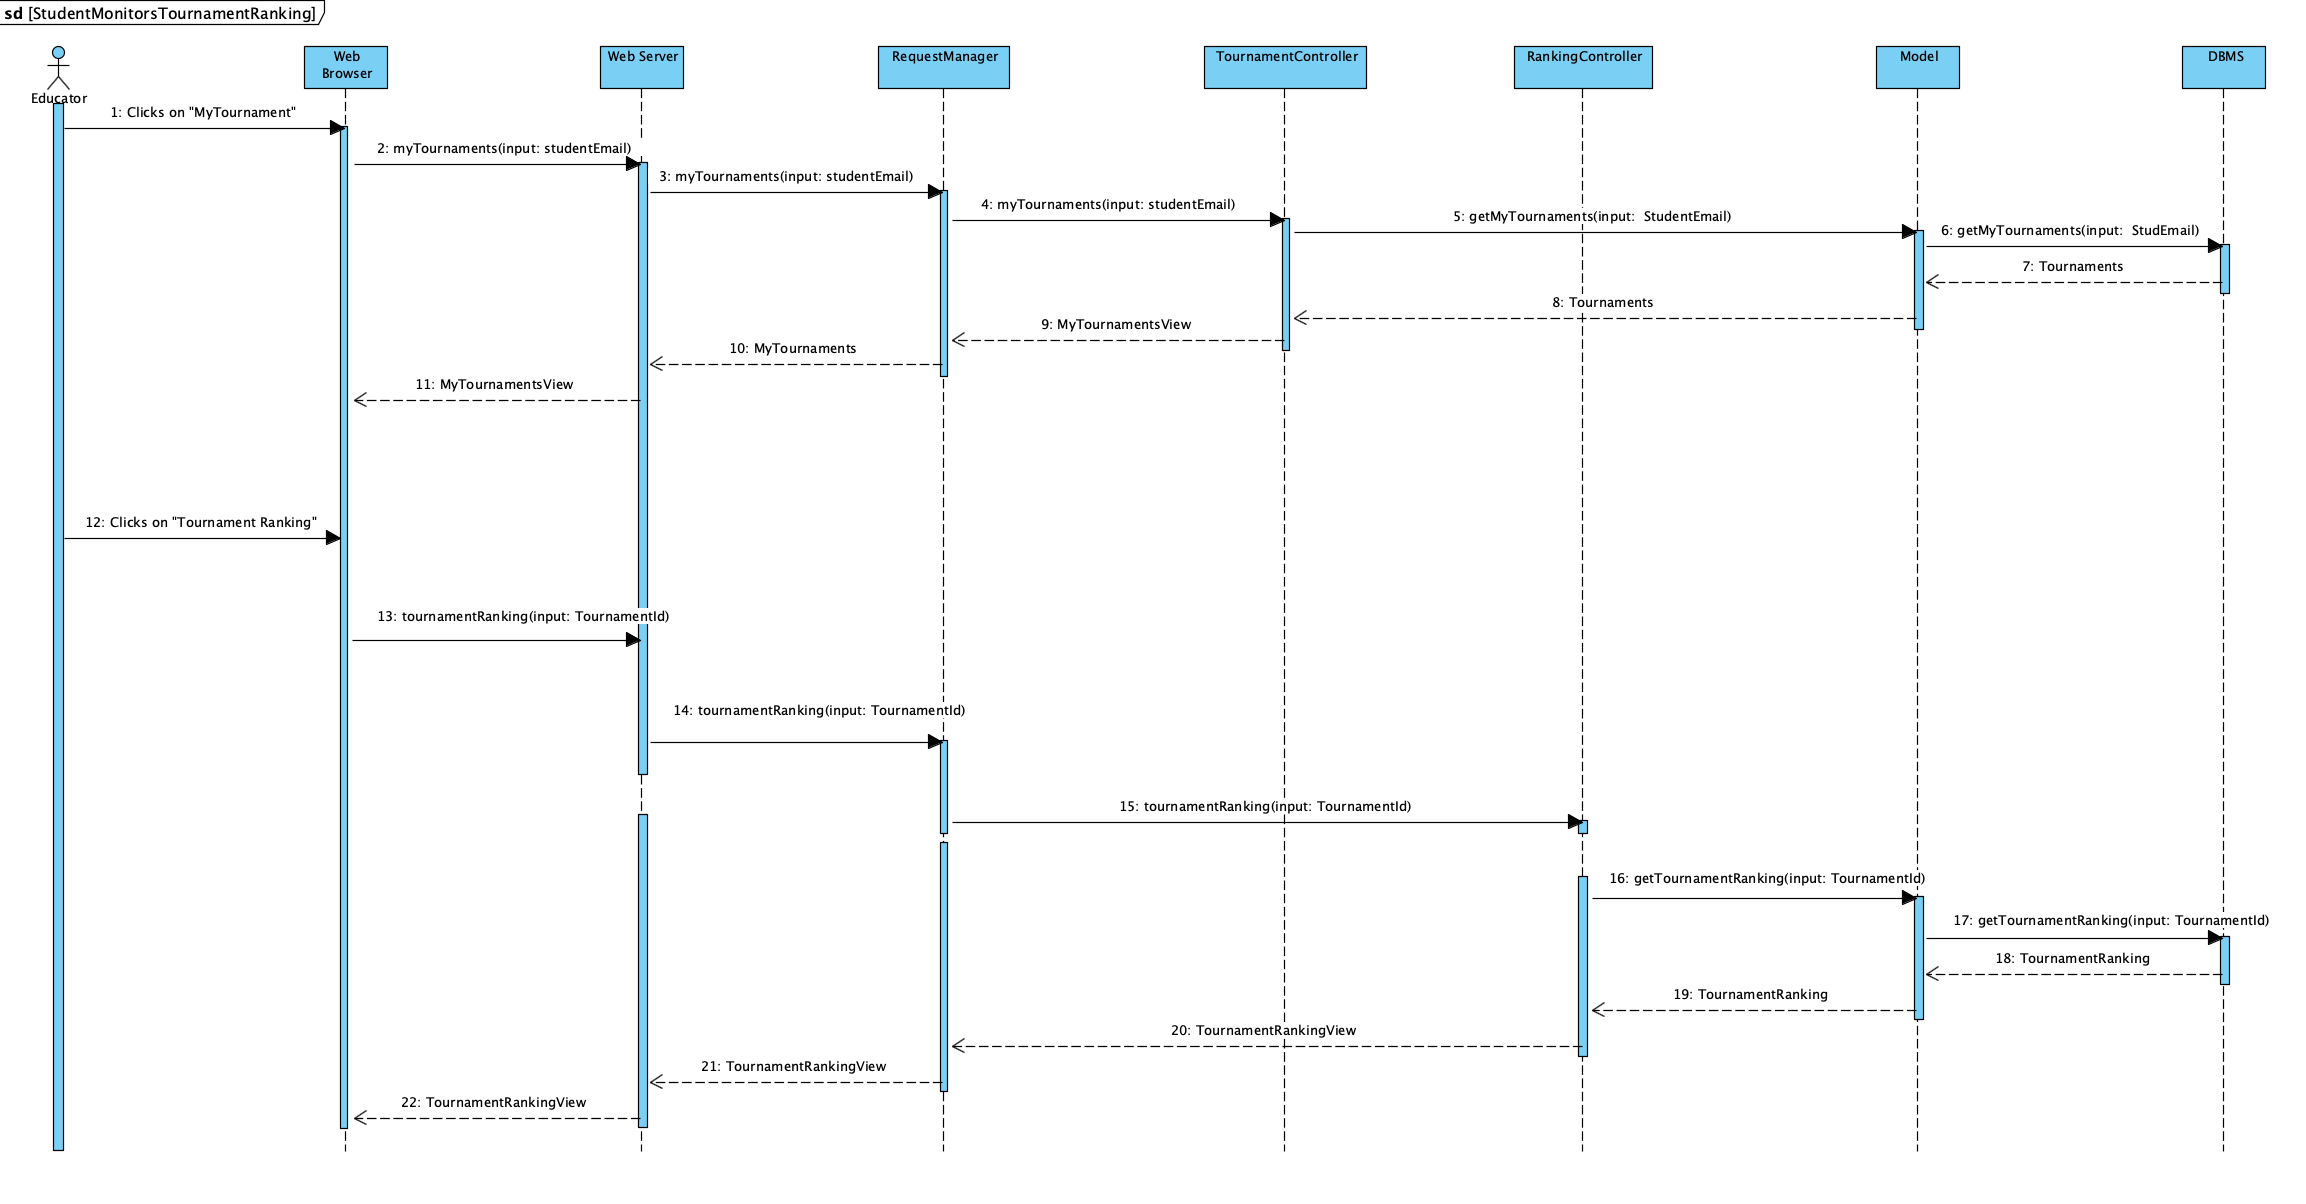
\includegraphics[width=1\textwidth]{SequenceDiagram/StudentMonitorsTournamentRanking.png}
    \label{fig:enter-label}
\end{figure}
In the sequence diagram, a student follows a procedure to view the ranking of a tournament within CKB.
It all starts on the homepage, where the student clicks on the "Tournaments" section, triggering a series of requests through the platform. The first request is sent from the student's web browser to the web server, which then forwards it to the Request Manager. The Request Manager, acting as the request distributor, sends the appropriate request to the Tournament Controller.
The Tournament Controller is the module responsible for retrieving the list of tournaments the student is a member of or has allowed to view, interacting with the Model to obtain this data from the Database Management System. The available tournaments are then presented to the student in a control view.
When the student selects a specific tournament, the system displays a page with the battles for that tournament and provides a button to view the tournament standings. By clicking on the "Tournament Ranking" button, the system, through the same backend interactions, requests the Ranking Controller to retrieve the rankings for the selected tournament.
The Ranking Controller, using the Model and interacting with the DBMS, obtains the current rankings. This information is then passed back through the system and displayed to the student.

%%%%%%%%%%%%%%%%%%%%%%%%%%%%%%%%%%%%%%%%%%%%%%%%%
\subsubsection{Tournament Closure}
\begin{figure}[H]
    \centering
    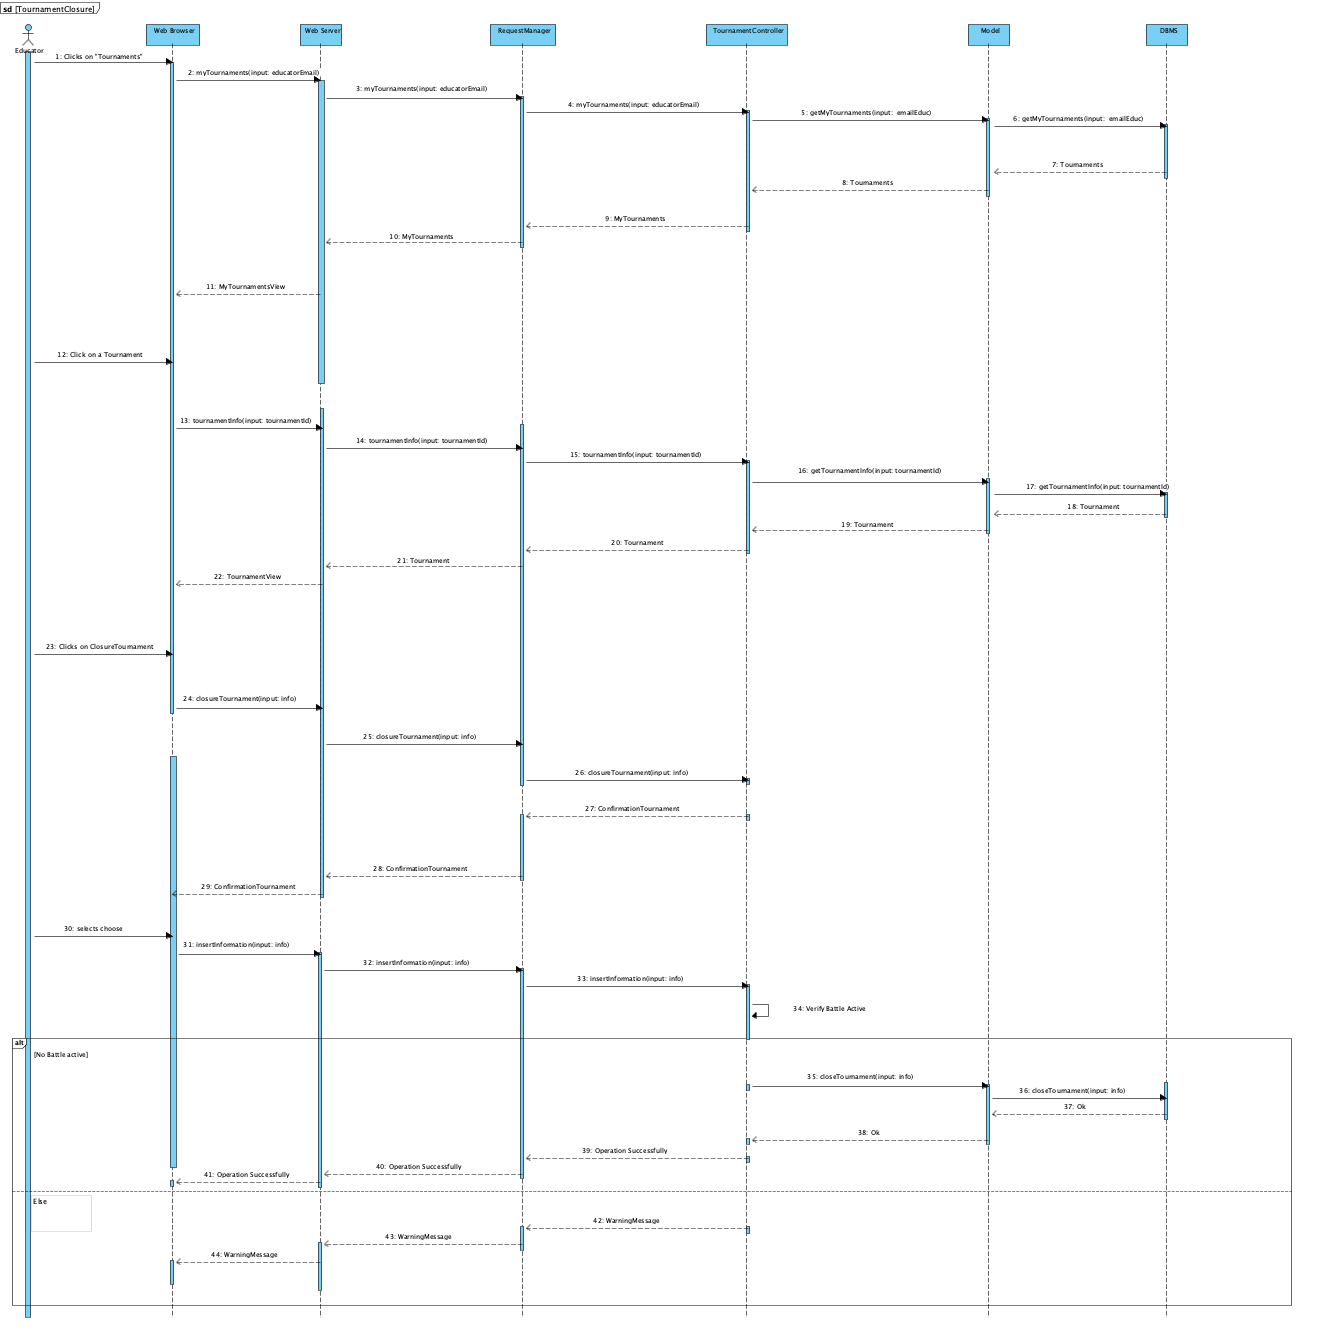
\includegraphics[width=1\textwidth]{SequenceDiagram/TournamentClosure.png}
    \label{fig:enter-label}
\end{figure}
In this scenario, the educator takes a series of actions on the platform to close a tournament. After
selecting the ’Tournaments’ section from the homepage, a control dashboard is displayed through his
web browser. This dashboard is the result of a series of interactions between the browser, the web server,
and the Request Manager, which coordinates incoming requests. The Request Manager forwards the
tournament display request to the Tournament Controller. The Tournament Controller then interacts
with the Model to extract the tournament data from the Database Management System (DBMS). When
the educator chooses to close a tournament by clicking on the ”Close Tournament” button, the system
displays a confirmation message to ensure that the intention is deliberate and not an accidental action.
If the educator confirms the closure, the system performs a check via the Tournament Controller to see if
there are any battles still open in the tournament. If there are no open battles, the Tournament Controller
sends a command to the Model to change the tournament status from ’Open’ to ’Closed’ in the DBMS.
The Model updates the DBMS with the new status and, once the DBMS confirms that the operation
has been successfully performed, the system informs the educator that the closing of the tournament
has been successfully completed. This feedback is provided directly through the user interface in the
educator’s dashboard.
24


%%%%%%%%%%%%%%%%%%%%%%%%%%%%%%%%%%%%%%%%%%%%%%%%%
\subsubsection{Battle elimination}
\begin{figure}[H]
    \centering
    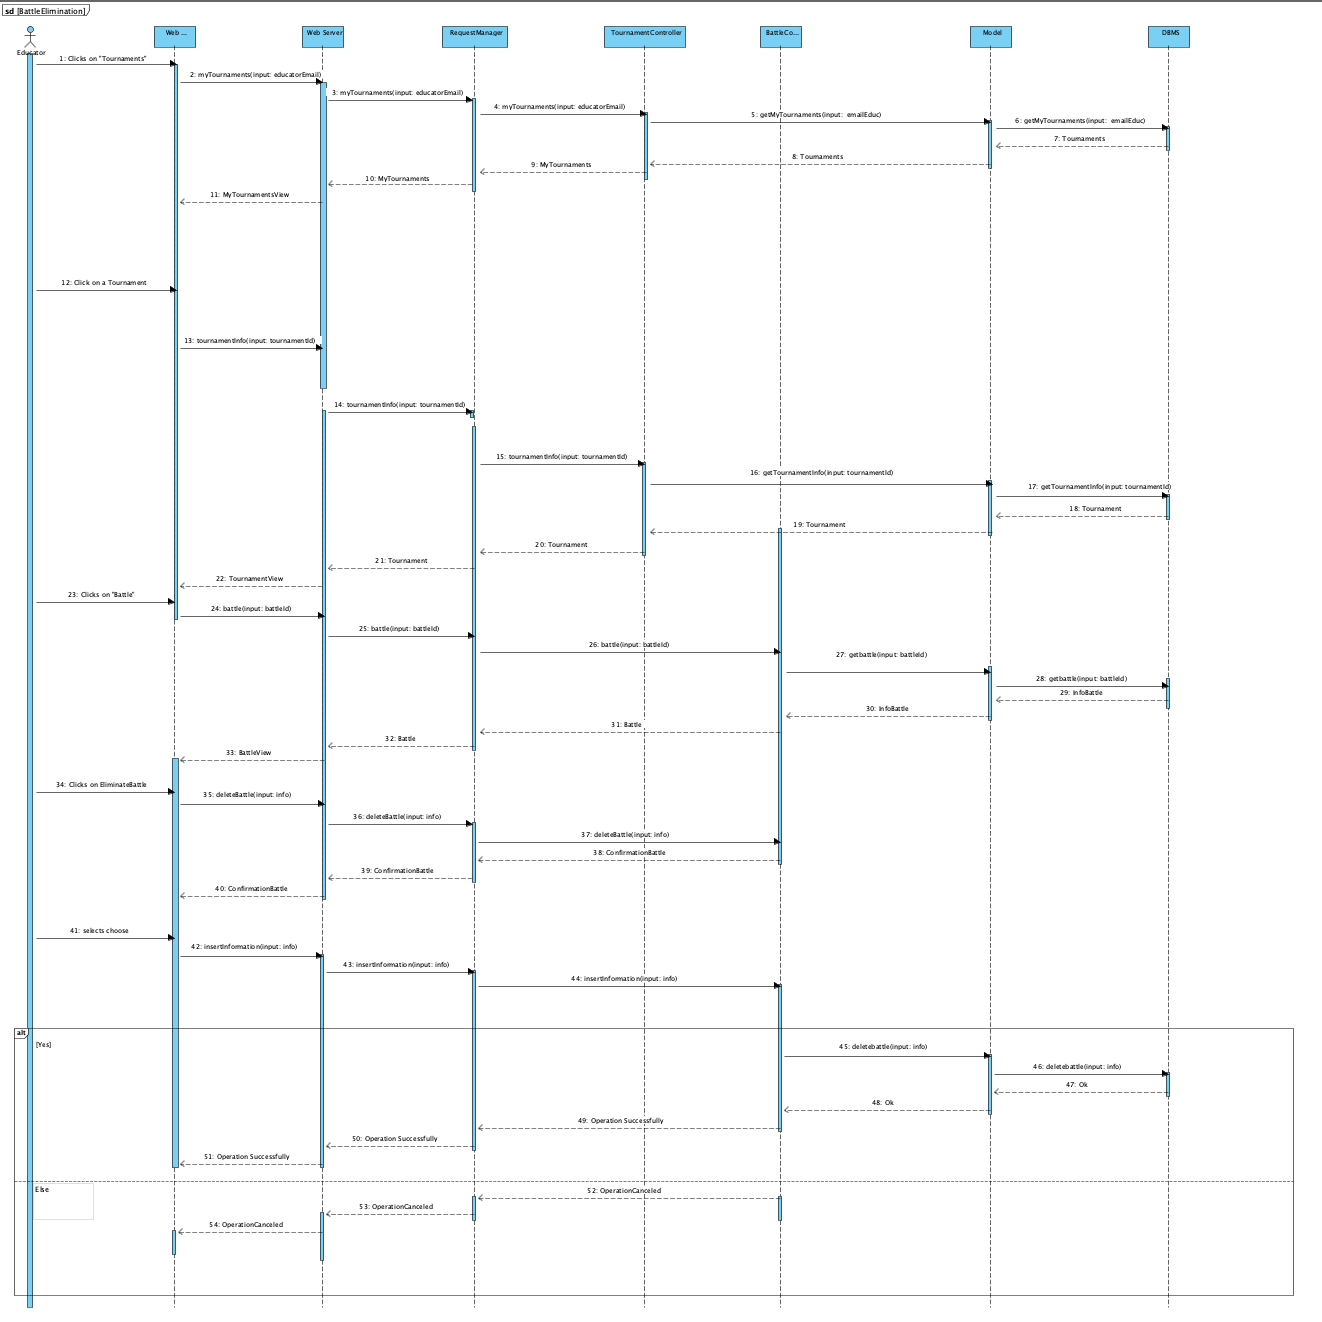
\includegraphics[width=1\textwidth]{SequenceDiagram/BattleElimination.png}
    \label{fig:enter-label}
\end{figure}
In the sequence diagram, the educator begins the process of eliminating a battle within a tournament. Once the "Tournaments" section has been clicked, the web server processes the request and via the Request Manager directs it to the Tournament Controller, who retrieves the list of available tournaments from the interaction with the Model and the Database Management System (DBMS).
By selecting a specific tournament, the educator accesses the tournament dashboard where the various battles are listed. The system, again through the Tournament Controller, shows the detailed page of the selected tournament and presents the option to "Delete the battle". The latter allows the educator to proceed with the elimination.
When the educator chooses to delete a battle, the system presents a confirmation message to ensure that they wish to proceed. This confirmation is processed once again by the web server and the Request Manager, which send the request to the Battle Controller.
After the educator's confirmation, the Battle Controller checks the battle status. If the battle can be deleted, the Battle Controller proceeds with the deletion request to the DBMS. The DBMS performs the deletion and sends a confirmation response to the Model, which in turn informs the Battle Controller of the deletion.
Ultimately, the educator receives visual feedback via the web browser displaying the message “Elimination Completed Successfully,” indicating that the battle has been removed from the database and that the tournament has been updated to reflect this change.
If the educator clicks no, the operation is canceled.
%%%%%%%%%%%%%%%%%%%%%%%%%%%%%%%%%%%%%%%%%%%%%%%%%
\subsubsection{Tournament Elimination}
\begin{figure}[H]
    \centering
    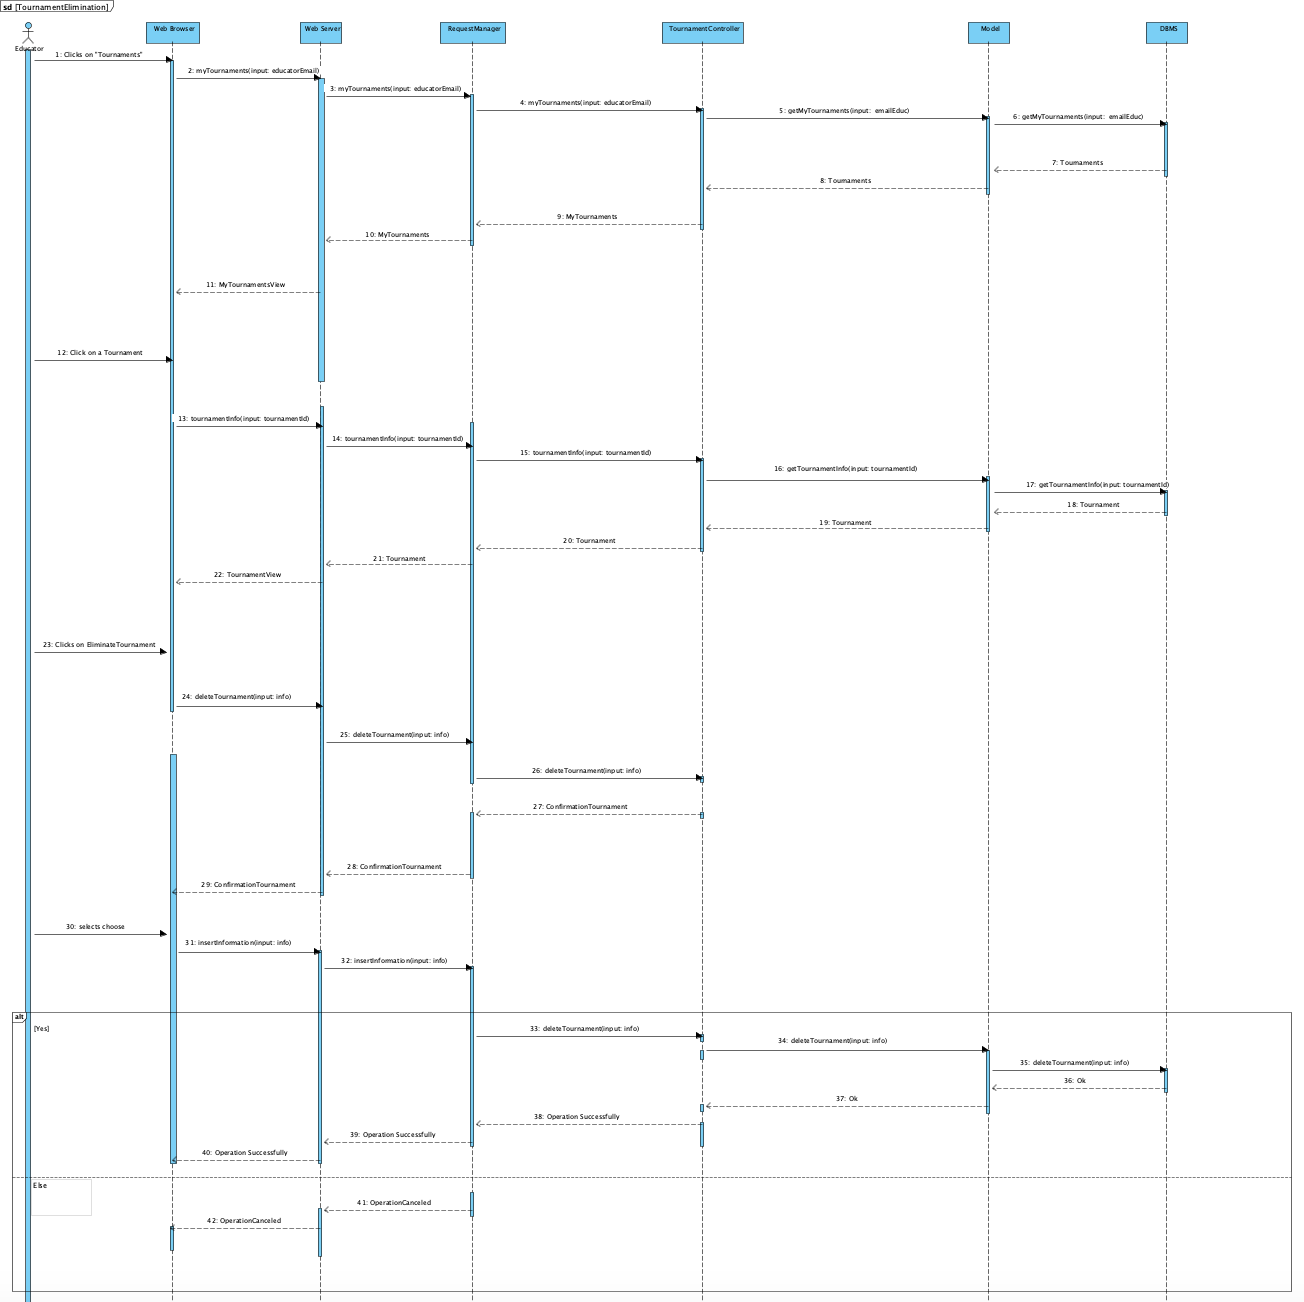
\includegraphics[width=1\textwidth]{SequenceDiagram/TournamentElimination.png}
    \label{fig:enter-label}
\end{figure}
In the sequence diagram, the educator uses the online platform to cancel an existing tournament. Start from the homepage, where you select the "Tournaments" section and are presented with a control dashboard listing all the tournaments available to you. This view is the result of a series of requests managed by the web server, which interacts with the Request Manager which forwards the request to the TournamentController which retrieves the data from the DBMS via the Model.
Once a specific tournament is chosen, the system displays a detailed page for that tournament via the Tournament Controller, which acts as an intermediary between the educator's request and the tournament information held in the system. The dashboard also includes a “Delete Tournament” button, which the educator can select to begin the cancellation process.
When the educator clicks "Delete Tournament", a warning message appears. By confirming your choice, the system triggers a check through the Tournament Controller to ensure that there are no battles still ongoing within the tournament.
If there are no obstacles, the system proceeds with the elimination of the tournament. This step involves the Model, which interacts with the Database Management System (DBMS) to update the tournament status. The DBMS performs the tournament cancellation and reports the completed operation to the model.
Finally, the system confirms the elimination of the tournament to the educator, displaying a confirmation message on the web browser. This signals that all changes have been successfully made in the database and that the tournament has been permanently removed from the platform.
%%%%%%%%%%%%%%%%%%%%%%%%%%%%%%%%%%%%%%%%%%%%%%%%%

\subsection{Component interfaces}

\begin{itemize}
    \item \textbf{LoginManager}: This component offer, through interface VisitorInterface this functions:
    \begin{enumerate}
        \item registration/login()
        \item login(input: email, password)
        \item logout()
    \end{enumerate}
    \item \textbf{SignupManager}: This component offer, through interface VisitorInterface this functions:
    \begin{enumerate}
        \item registration/login()
        \item signup(input: name, surname, email, password, userType)
    \end{enumerate}
    \item \textbf{BattleManagementController} : This component offer, through interface StudentInterface this functions:
    \begin{itemize}
        \item battle(input: battleId)
        \item createTeam(input: emailCreator, battleId)
        \item joinTeam(input: teamId, battleId, emailUser)
      %  \item joinBattle(input: teamId, battleId)
        \item initiateRegistration(input: battleId)
        \item insertInformationTeam(input: emailStudent[],info)
    \end{itemize}
    \item \textbf{BattleManagementController}: This component offer, through interface EducatorInterface this functions:
    \begin{enumerate}
        \item insertInformation(input: info)
        \item deleteBattle(input: battleId, emailEducator, tournamentId)
         \item createBattle(input: battleInfo, emailEducator, tournamentId)
        \item deleteBattle(input: battleId, emailEducator, tournamentId)
        \item battle(input: battleId)
        \item getSubmissionProjects(input: battleId)
        \item getProject(input: projectId,battleId)
    \end{enumerate}
  \item \textbf{TournamentController}: This component offer, through interface StudentInterface this functions:
  \begin{enumerate}
       \item tournamentInfo(input: tournamentId)
      \item  joinTournament(input: tournamentId, emailStudent)
      \item tournaments()
      \item myTournaments(input:studentEmail)
  \end{enumerate}
\item \textbf{TournamentController}: This component offer, through interface EducatorInterface this functions:
\begin{enumerate}
        \item insertInformation(input: info)
    \item tournaments()
    \item myTournaments(input: educatorEmail)
   \item tournamentInfo(input: tournamentId)
    \item createTournament(input: tournamentInfo)
    \item deleteTournament(input: tournamentId, emailEducator)
    \item closureTournament(input: tournamentId, emailEducator) 
      \item verifyBattleActive()
\end{enumerate}
\item \textbf{RankingController}: This component offer, through interfaces StudentInterface and EducatorInterface this functions:
\begin{enumerate}
    \item battleRanking(input: battleId)
    \item tournamentRanking(input: tournamentId)
    \item calculateRanking()
\end{enumerate}
\item \textbf{ManualEvaluationController}: This component offer, through interfaces EducatorInterface this functions:
\begin{enumerate}
    \item submitEvaluation(scores[])
    \item downloadProject(input: projectId)
\end{enumerate}
\item \textbf{AutomatedEvaluationController}: This component offer,  this functions:
    \item computeScoreTeam(input: teamId)
\begin{enumerate}
    \item setEvaluation(input: parameters, Project)
\end{enumerate}
\item \textbf{NotificationManager}:
\begin{enumerate}
    \item sendEmail(input: emailUser, content)
\end{enumerate}
\item  \textbf{Model}:
\begin{enumerate}
    \item addInfoTournament(input: tournamentInfo, emailEducator)
    \item getMyTournaments(input: emailEducator)
    \item getTournamentInfo(input: tournamentId)
    \item addInfoBattle(input: info)
    \item getTournaments()
    \item getTeamMemberBattle(input: idBattle)
    \item joinTournament(input: tournamentId,emailStudent)
    \item getBattle(input: battleId)
    \item addToTeam(input:teamId, battleId, emailUser)
    \item updateScore(input: teamId,score)
    \item getSubmissionProjects(input: battleId)
    \item getProject(input: projectId, battleId)
    \item setSubmitEvaluation(input: scores[])
    \item insertRanking(input:ranking, battleId)
    \item getBattleRanking(input: battleId)
    \item getTournamentRanking(input: tournamentId)
    \item closeTournament(input: tournamentId, emailEducator)
    \item getAllTournaments()
    \item  deleteBattle(input: battleId, emailEducator, tournamentId)
    \item deleteTournament(input: tournamentId, emailEducator)
\end{enumerate}
\item \textbf{WebServer}:\begin{enumerate}
    \item registration/login()
    \item login(input: email, password)
    \item signup(input: userInfo)
    \item myTournaments(input: educatorEmail)
    \item createTournament(input: tournamentInfo)
    \item createBattle(input: battleInfo, emailEducator, tournamentId)
    \item tournaments()
    \item tournamentInfo(input: tournamentId)
    \item joinTournament(input: tournamentId, emailStudent)
    \item battle(input: battleId)
    \item initiateRegistration(input: battleId)
    \item createTeam(input: emailCreator, battleId)
    \item insertInformationTeam(input: emailStudent[],info)
    \item sumbissionProjects(input: battleId)
    \item project(input: projectId, battleId)
    \item downloadProject(input: projectId, battleId)
    \item submitEvaluation(input: scores[])
    \item tournamentRanking(input: tournamentId)
    \item closureTournament(input: tournamentId, emailEducator) 
    \item insertInformation(input: info)
    \item deleteBattle(input: battleId, emailEducator, tournamentId)
    \item deleteTournament(input: tournamentId, emailEducator)
\end{enumerate}

\end{itemize}

\subsection{Architectural Styles and patterns}
\subsubsection{Four-tier system architecture}
This system has a 4 tiers architecture. The benefit from this choice are:
\begin{itemize}
    \item \textbf{Scalabilità}: Con i componenti logicamente divisi, è più semplice scalare il sistema. Se, per esempio, il carico sul server web aumenta, puoi aggiungere più server web senza modificare gli altri tier.
    \item \textbf{Flessibilità}:Ogni tier può essere modificato, aggiornato o sostituito indipendentemente dagli altri.
\end{itemize}
\subsubsection{RESTful architecture
}
The choice of a RESTful architecture for communication with the application server offers several advantages:
\begin{itemize}
    \item \textbf{Simplicity and Standardization}: REST uses standard HTTP methods, which are understood by developers and supported by virtually all web infrastructure. 
    \item \textbf{Scalability}:the stateless nature of the server leads simplifies upkeep, allowing for the addition or migration of a server without altering any data
    \item \textbf{Independence}: The client and the server are independent; the client doesn't need to know anything about the business logic, and the server doesn't need to know anything about the UI. This separation allows for the client and the server to evolve independently.
\end{itemize}
\subsubsection{Model View Controller}
Model-View-Controller (MVC) architecture was chosen for the development of your web application. It includes:
\begin{itemize}
    \item \textbf{Model}: Questa parte gestisce i dati e le regole dell'applicazione, offrendo metodi per manipolare questi dati.
    \item \textbf{View}: È responsabile della presentazione visiva dei dati. Può esistere in molteplici forme, consentendo diverse rappresentazioni dell'informazione a seconda delle necessità dell'utente.
    \item \textbf{Controller}: Funziona come mediatore tra Model e View. Risponde agli eventi, come l'interazione dell'utente con l'interfaccia (ad esempio, la pressione di un pulsante), elaborando i dati nel Model che poi saranno riflessi nella View.
\end{itemize}

\subsection{Other design decisions}
In this part, we discuss various design choices implemented in the system to ensure its optimal functioning.
\subsubsection{Availability}
We have added load balancing and replication to make the system more reliable and to keep it running smoothly. This means if one part has a problem, the system can still work because it has backups and shares the work. This helps to make sure the system can handle data safely and stay available for use without interruption.


